% Fine detection of grasp force and posture by amputees via surface electromyography
% Castellini, Gruppioni, Davalli, Sandini
% accepted by Journal of Physiology, Paris --- Special issue on Neuro-robotics
%
% March, 2009

\documentclass[review,authoryear]{elsarticle}

\usepackage{times}
\usepackage{epsfig}
\usepackage{graphicx}
\usepackage{amsmath}
\usepackage{amssymb}
\usepackage{url}

\def\RR{\mathbb{R}}
\def\NN{\mathbb{N}}
\def\xx{\mathbf{x}}
\def\yy{\mathbf{y}}
\def\ww{\mathbf{w}}

\def\re{\textsf{re}}
\def\po{\textsf{po}}
\def\pw{\textsf{pw}}
\def\pi{\textsf{pi}}
\def\tr{\textsf{tr}}
\def\hs{\textsf{hs}}

\renewcommand{\cite}{\citep}

\journal{J Physiol Paris}

\begin{document}

\begin{frontmatter}

\title{Fine detection of grasp force and posture\\
by amputees via surface electromyography}

\author[liralab]{Claudio Castellini\corref{corauth}}
\ead{claudio.castellini@unige.it}
\author[inail]{Emanuele Gruppioni}
\ead{e.gruppioni@inail.it}
\author[inail]{Angelo Davalli}
\ead{a.davalli@inail.it}
\author[iit]{Giulio Sandini}
\ead{giulio.sandini@iit.it}

\address[liralab]{LIRA-Lab, University of Genova,
  viale F. Causa 13, 16145 Genova (Italy)}
\address[inail]{INAIL Centro Protesi,
  via Rabuina 14, 40054 Vigorso di Budrio (Bologna, Italy)}
\address[iit]{RBCS Department, Italian Institute of Technology,
  via Morego 30, 16163 Genova (Italy)}

\cortext[corauth]{Corresponding author}

\begin{abstract}

The state-of-the-art feed-forward control of active hand prostheses
is rather poor. Even dexterous, multi-fingered commercial prostheses are
controlled via surface electromyography (EMG) in a way that enforces
a few fixed grasping postures, or a very basic estimate of force.
Control is not natural, meaning that the amputee must learn to associate,
e.g., wrist flexion and hand closing. Nevertheless, recent literature
indicates that much more information can be gathered from plain, old
surface EMG. To check this issue we have performed an experiment in
which three amputees train a Support Vector Machine (SVM) using five
commercially available EMG electrodes while asked to perform various
grasping postures and forces with their phantom limbs. In agreement
with recent neurological studies on cortical plasticity, we show that
amputees operated decades ago can still produce distinct and stable
signals for each posture and force. The SVM classifies the posture up
to a precision of $95\%$ and approximates the force with an error of
as little as $7\%$ of the signal range, sample-by-sample at $25$Hz.
These values are in line with results previously obtained by healthy
subjects while feed-forward controlling a dexterous mechanical hand.
We then conclude that our subjects could finely feed-forward control
a dexterous prosthesis both in force and position, using standard EMG
in a natural way, that is, using the phantom limb.

\end{abstract}

\begin{keyword}
  learning and adaptive systems \sep
  support vector machines \sep
  hand prosthetics \sep
  electromyography \sep  
\end{keyword}

\end{frontmatter}

\section{Introduction}
\label{sec:intro}

As of today, the most common way of feed-forward controlling an active
hand prosthesis is via forearm surface electromyography (EMG),
a technique by which motor unit activation potentials are read from the
amputee's stump skin and then used to command the prosthesis \cite{deluca97}.
The clinical success of EMG is motivated by its non-invasiveness and
relatively low cost \cite{englehart06}.
Still, even though multifingered hand prostheses have appeared on the market
(for example Touch Bionics's i-LIMB, see \url{www.touchbionics.com}),
it seems that EMG-based control is not keeping the pace, being limited to a
few hand postures or a simple proportional estimate of force.
Moreover, this control is quite non-natural, meaning that the amputee must
learn to associate muscle remnants actions to unrelated postures of the
prosthesis, e.g., phantom wrist flexion and hand closing.

It would be desirable, for a dexterous prosthesis, to let the amputee command a
grasp posture and force just by performing the corresponding action with the
phantom limb, resulting in a movement or force elicited by "desiring"
it. Also, a way to finely modulate the force involved in a grasp is paramount
in daily life activities, for example to hold an egg without breaking it or to
grasp a hammer without letting it slip. Lastly, the system should be able to
work in real-time and to adapt continually to the changing nature of the EMG
signal.

Actually, recent scientific literature indicates that plain, old EMG signals
can be used in a better way in prosthetics, by improving the signal processing
method, essentially by switching to machine learning. Excellent results have
been shown on healthy subjects, but surprisingly, as far as we know, there is
so far just one study on amputees \cite{sebelius}. Willing to explore the issue
deeper and further, we have devised a new experiment. Three below-elbow traumatic
amputees, two of which were operated decades ago, were asked to perform
grasp postures with their phantom limb at various speeds and forces, while their
EMG activity was recorded using $5$ commercially available electrodes, positioned
without clinical help, and the desired force was
estimated using a force sensor in three different ways.
The EMG and force signals were used to train a standard machine learning system
(a Support Vector Machine) in order to check how well phantom limb postures
could be discriminated and the required force approximated. This paper is
a report of the experiment, whose outcome is positive.

We now quickly revise related work highlighting the novel contributions of this
work, then we describe the experiment and results and discuss them.

\subsection{Related work}

\subsubsection{Myoelectric control}

Myoelectric control, i.e., feed-forward control of prostheses using surface EMG,
is in use since the Sixties to control (externally powered) upper-limb prostheses
by amputees mostly due to its relatively low cost and non-invasiveness. It
provides a simple yet effective way to control single degree-of-freedom (DOF) hand
prostheses such as OttoBock's SensorHand for decades, also allowing for a simple
force estimation, the so-called proportional control. Before 1975, the common
control schema was based upon the identification of active muscle remnants in the
amputee's stump and the coding of two, at most three levels of activity of each
remnant to prosthesis commands, e.g. \cite{bottomley65,childress69}. From the mid-Seventies
on probabilistic methods and pattern recognition techniques began to be used,
including Bayes methods, artificial neural networks and nearest neighbors. 
A thorough and well-organised survey and historical account of myoelectric
control for hand prostheses can be found in \cite{englehart06}.

With the appearance on the market of multiple-DOFs hand prostheses, the myoelectric
signal gains even more interest, since it represents the only non-surgical
way of finely controlling such artifacts. \cite{englehart01,dunlop,smagt06} are
examples of better and better posture discrimination using EMG, always on healthy
subjects. The issue is important also outside the field of prosthetics, e.g., in
robotic control and teleoperation \cite{fukuda,yokoi}.

In \cite{2008.ICRA,2008.BioCyb} it has been verified on one single healthy subject
that the problem, from the very point of view of machine learning,
is easy, and that a Support Vector Machine \cite{BGV92},
a standard multi-layer perceptron and an incremental local-approximation
method such as LWPR \cite{lwpr} obtain similar results when applied to the plain EMG
signal as extracted by Otto Bock's commercially standard electrodes, the Myobock
(see \url{www.ottobockus.com}).

It seems then reasonable to say that surface myoelectric control will still be the
standard for the years to come, even when the dexterity of commercial prostheses
increases. Single-DOF control via EMG is being studied \cite{englehart08} and looks
extremely promising. As many as $127$ EMG electrodes are used simultaneously in Targeted
Muscle Reinnervation \cite{kuiken06}, probably the most spectacular use of myoelectric control
so far, although it is out of the scope of this work since it involves surgery.

\subsubsection{Artificial / prosthetic hands}

In Section $3$ of \cite{zecca02} a full comparison among artificial hands, including
the human hand, is shown; remarkable mechanical hands such as the Utah/MIT hand, the
Stanford/JPL hand, the DLR hand and the Robonaut Hand are compared (see also the
references in the paper for more details); but in those cases high dexterity means they
are not usable as prostheses, either because they are too large, too heavy or too power-demanding.
As well the DLR-II hand, appeared in 2004 \cite{ButFisGre2004}, probably the most sophisticated
mechanical hand at the time of writing, is far from being usable as a prosthesis.

As of 2004, a widely employed prosthesis was the Otto Bock / SUVA hand, which only had $2$ DOFs and
no opposable thumb. More recently, Touch Bionics's i-LIMB (\url{www.touchbionics.com}) has appeared, which has
5 independent DOFs and a passive opposable thumb. Its myoelectric control system enables
the selection among $5$ hand postures using $2$ electrodes (information collected from the
website); nevertheless, the impression is that most of the grasping effort is achieved through
the underactuation of the hand, as it happens with the CyberHand \cite{cyberhand}, still at
the prototype level, and the DLR Prosthetic Hand \cite{Hua2006}. Force control is a hot topic
currently being studied in robotics \cite{ott,thomas} as well as in hand prosthetics, among others
in \cite{meek1,meek2}. There is a definite trend of transferring technology from
mechatronics to prosthetics and we are probably going to see more and more dexterous
prostheses built and marketed in the upcoming years; still, control
lags behind, even without considering the crucial issue of sensorial feedback,
dealt with in, e.g., \cite{cipriani} but completely open as yet.

\subsubsection{Clinical applications}

All aforementioned works and systems have been tested on healthy subjects. At the time
of writing and to the best of our knowledge, \cite{sebelius} is the only test on amputees, done
in the framework of Project SmartHand (\url{www.elmat.lth.se/~smarthand}).
Sebelius had $5$ below-elbow amputees, plus one subject
with congenital malformation of the forearm, perform up to
$10$ hand postures (not grasping-related) while recording a 16-channel EMG signal. His
results indicate that a rather high recognition rate is obtained by a neural network
aided by a sort of decision tree, although not uniformly for all subjects; and that
the age of amputation seems not to influence the subjects' ability.

\subsubsection{Original contributions}

To the best of our knowledge, this is the first time a position / force estimation
is attempted on amputees somehow systematically. We apply a standard machine learning
system to the EMG of three amputees both to recognise the grasping posture and
to approximate the required force. Some considerations about the subjects' diversity
as patients (age, age of operation, type of amputation) are drawn, also with respect to
its impact on the results. Just $5$ commercially available EMG electrodes are
employed, and their signals are directly fed to the machine at $25$Hz;
classification and regression are performed sample-by-sample.
(Traditionally, isometric/isotonic postures are classified after a certain amount
of signal has been presented to the system, which introduces delay --- this issue
has recently been tackled in \cite{tsukamoto}, too.) The encouraging results,
and the simplicity of the tools used, indicates that surface EMG still has to be
fully exploited.

\section{Materials and Methods}
\label{sec:m&ms}

\subsection{Subjects}

Three hand amputees, patients of the INAIL Centro Protesi in Vigorso
di Budrio, Bologna, Italy, joined the experiment voluntarily after
having been carefully informed of the procedure they were about to undergo,
according to the INAIL patients care guidelines. All of them have lost
their limb traumatically and, at the time of the experiment, the status of
their muscle remnants was excellent.

Subject $1$ is male, 63 years old, trans-radial
one-third proximal, amputated in 1963; he is a
pioneer of myoelectric prostheses, having started using them in the
Sixties. The Subject $2$ is male, aged 56, trans-radial one-third
distal, amputated in 1972; he also started using myoelectric prostheses
very early, actually in 1974. Subject $3$ is male as well, aged 25,
trans-carpal, amputated in 2007; he was in the process of learning how
to use a standard myoelectric prosthesis at the time the experiment was
performed (summer 2008). Subject $1$ has about $9$cm left of his
forearm, Subject $2$ has some $20$cm, and Subject $3$ has the whole forearm
plus some of the carpus --- see Figure \ref{fig:stumps}.

\noindent \textbf{[Figure \ref{fig:stumps} about here]}

\subsection{Setup}

\noindent \textbf{[Figure \ref{fig:setup} about here]}

We used a FUTEK LMD500 Hand Gripper force sensor \cite{futek}, a strain-gauge
based sensor with guaranteed low non-linearity and hysteresis factors, which can easily
be gripped in various ways since it is light and small. The sensor returns a
voltage proportional to the force applied to its narrow face (Figure \ref{fig:setup}, left).
Also, $5$ standard commercial surface EMG electrodes were used, namely OttoBock
Myobock models \cite{myobock}, type 13E125=50 (Figure \ref{fig:setup}, center).
The electrodes are dry bi-differential with a frequency bandwidth ($-3$dB) of
$140$-$1500$Hz, adjustable amplification gain from $0$ to $50000$, CMMR of
$80$dB and a double T notch filter at $50$Hz (in the European version
that we used) for power supply interference rejection. After a few initial
experiments, we set the amplification at mid-range, which gave us an output voltage
exactly matching the input range of the acquisition card.
These electrodes are the state-of-the-art in commercially available myoprostheses,
since their output is deemed exceptionally good, highly correlated with the
force exerted by the muscle(s) whose activity the electrode is gathering.
All in all, six signals were monitored (one per each EMG electrode and one from the
force sensor), and sampled at a rate of $100$Hz via a standard USB acquisition card,
connected to an entry-level laptop.

The electrodes were placed around the stump just below the elbow, parallel
to the forearm axis, equally spaced and held in place by an elastic band
(Figure \ref{fig:setup}, right panel). This was done
in order to detect signals from all muscle remnants uniformly,
rather than try and associate electrodes to single muscles
as is the case in normal one-DOF myodevices. By the way, for Subject $1$
this was the only possibility, since his stump
would not allow the electrodes to be positioned anywhere else --- this problem
of ``cluttered'' electrodes on a subject's stump actually also appears in
\cite{sebelius}.

\subsection{Experimental procedure}

\subsubsection{Grasping postures}

The subjects were asked to perform with their phantom hand several
different grasp postures, chosen according to suggestions by the
INAIL Centro Protesi personnel and patients, and loosely based upon
Cutkosky's taxonomy \cite{cutkosky}:

\begin{enumerate}

  \item the baseline \emph{rest condition} (\re);

  \item the act of \emph{pointing the index finger} (\po), used when pressing buttons;

	\item a \emph{power grasp} (\pw) in which the whole hand wraps around an object,
		used, e.g., when holding a heavy cylindrical object such as a hammer;
		
	\item a \emph{precision pinch grip} (\pi) with thumb and index finger closing on
	 	an object, usually for lifting small objects such as a pen or an egg;
	
	\item a \emph{precision tripodal grip} (\tr) similar to \pi, but using the
		middle finger too, used for spherical objects;
		
	\item the act of \emph{stretching one's hand} (\hs), used when an amputee is trying
		to put his hand inside a pocket. 

\end{enumerate}
	
Each posture was performed repeatedly by each subject a free number of times,
ranging from $10$ to about $25$ (except the rest condition, obviously, which consisted
of a few seconds of no-activity recording), with speeds ranging from $5$Hz to
"slow motion" (about $20$ seconds to complete a grasp, using various degrees of
force). The postures were performed in the order described
above, with a few seconds of rest inbetween. The
experimenter would at times suggest the subject to go faster or slower, to press
harder or softer, and at times the subject would be free to do whatever he wanted.
We will call this sequence a \emph{cycle}.

\subsubsection{Training modalities}

Since we employ a supervised learning strategy, a way of knowing what the subject is
doing is required in the training phase. In particular, each sample must be associated
to a label, denoting the current grasp posture, and to a force value.

Labels, one for each required posture (\re,\po,\pw,\pi,\tr,\hs),
were attached to each sample simply according to the
type of grasp required from the subject during a particular phase of the current
cycle; for example, samples gathered while asking the subject to perform a power grasp
would be labled with \po, and so on.

Force values, on the other hand, were collected according to three
\emph{modalities} (see Figure \ref{fig:modalities}):

\begin{enumerate}

  \item \emph{teacher imitation.} A healthy subject (the teacher)
    would place his arm besides the subject's stump and ask him
    to imitate the teacher's postures with his phantom limb. The
    subject was asked to grasp with maximum strength,
    while the teacher would grip the force sensor in order to mark the
    postures / grips.

  \item \emph{bilateral action.} The subject would grip the
    force sensor with his healthy hand while doing the same
    thing with the phantom limb.

  \item \emph{mirror-box.} Same as modality $2$, but a \emph{mirror-box}
    \cite{mirror-box} was used.

\end{enumerate}

\noindent \textbf{[Figure \ref{fig:modalities} about here]}

Each subject performed one cycle in each modality, resulting in a total
of nine cycles, with a length of $5.7 \pm 1.06$ minutes (average
$\pm$ one standard deviation). After all cycles were recorded, samples
associated with force signal values lower than $0.01$V were artificially
given the label \re. This threshold was detected by visual inspection
of the signal, and checked by comparing it with the values during the 
baseline rest condition. Due to an error in the
experiment protocol, Subject $1$ did not record the pointing index
grasp during the second modality, and Subjects $1$ and $2$ did not
record the hand stretching posture.

Figure \ref{fig:examples} shows some sample force and EMG signals obtained
during the experiments. Notice that for Subject $3$, two electrodes (blue and
red curves) suffer of a non-null baseline and slowly drifting components,
later on determined to be due to sweat. This is common when dealing with
surface EMG \cite{deluca97,deluca02}.

\noindent \textbf{[Figure \ref{fig:examples} about here]}

\subsection{Data pre-processing and preliminary analysis}

Both force and EMG signals were digitally filtered
to remove high-frequency noise components (II order low-pass FIR filter
with cut-off frequency at $5$Hz). After filtering, spectral analysis
reveals that the relevant bandwidth of the
EMG signal, as recovered form the elctrodes, and of the force signal,
lies below $10$-$12$Hz, so both signals were subsampled at $25$Hz.

Principal Component Analysis (PCA) was applied to the $5$ EMG signals in
each cycle, revealing that they can be linearly reduced to two losing,
on average, only $7.7\% \pm 4.4\%$ of the signal variance. Although this
loss would probably hinder classification and regression, and therefore
the $5$-dimensional original signals were used later on, this reduction
enables us to visualise the samples, tagging them according to the labels
(and therefore according to the grasp), and to qualitatively check
how well the subjects can produce different EMG
patterns when they are asked to perform different grasping
actions. Figure \ref{fig:PCA} shows the results, according to each
subject and modality.

\noindent \textbf{[Figure \ref{fig:PCA} about here]}

As is apparent from the Figure, all subjects can produce distinct signals
according to the required type of grasp. In particular,
notice how two very similar grasp types, i.e.,
\pi\ and \tr, are qualitatively discernible on almost each graph.
Notice that PCA being so effective in reducing the
dimensionality of the EMG signals two does not imply that
two electrodes would suffice to obtain the same results. In fact, PCA coefficients
consistently show the same magnitude, meaning that each electrode
is required.

\subsection{Classification / regression method}
\label{subsec:method}

The good performance of Support Vector Machines (SVMs) applied to similar
problems is known since \cite{smagt06}. SVMs are
statistical learning machines \cite{v-edbed-82} which build an approximated map between
samples drawn from an input space (under the standard i.i.d. sampling hypothesis)
and a set of labels (classification) or a real value (regression).
The map is a weighted sum of basic functions chosen a priori
via the so-called kernel (hence the term \emph{kernel methods}), each of
which is centered on a sample.
The weights are found by minimising a cost functional which is the sum of
a loss function, punishing the error on the samples, and a regulariser, punishing
over-complex solutions. For a comprehensive tutorial on SVMs please refer to
\cite{Burges98,SmolaTut2004}.

Maps found by SVMs are sparse, meaning that some (practically, most) of the
weights found by minimisation are zero.
Those samples for which the weight is not zero, that is, those which actually
contribute to the map, are called \emph{Support Vectors}
(SVs), and their number is usually much smaller
than the total number of samples used in the training phase --- this is why
prediction with SVMs is in practice rather fast \cite{Cristianini00}. The
ratio between the number of SVs and the number of samples is then a good index
to measure how difficult a problem is: the smaller the ratio, the easier
the problem, indicating that a few samples are sufficient to
fully determine the map. In classification, this means that samples with different
labels are well separated in the input space; in regression, it means that a
simple relationship exists between the samples and the target values.
The sparsity of SVM models is extremely useful in our context, since
smaller models also mean higher chance of miniaturising them and using them
in pratice on a prosthesis.

In our case, the input space is $\RR^5$, one coordinate for each EMG
electrode; EMG signals are fed to the SVM as they are, sample by sample. The labels are
(a subset of) $\{\re,\po,\pw,\pi,\tr,\hs\}$ while the regression value is exactly the
force value as read from the force sensor. No feature extraction besides the low-pass
filtering is, therefore, employed on the signals.

As is standard, we use a Gaussian kernel both for classification and regression.
Multi-class classification is realised via the all-pairs schema,
in which a quadratic number of SVMs are trained to discriminate pairs of grasp
postures, and then a final decision is made according to a voting criterion.
Regression is done using the $\epsilon$-SVR technique, which neglects errors smaller
than a tolerance threshold $\epsilon>0$, here set at the default value of $0.1$.
Multi-class classification and $\epsilon$-SVR are
provided by \emph{libsvm} v2.83 \cite{ChangL01} in the Matlab wrapped version.

For classification, the performance index is the \emph{weighted accuracy},
that is the average of the percentages of correctly predicted labels of type
$i$, divided by the number of labels $i$ in the testing set:

$$ \sum_{i \in \{\re,\po,\pw,\pi,\tr,\hs\}}	\frac{c_i}{n_i} $$

\noindent where $n_i$ is the number of samples tagged with the label $i$
in the testing set and $c_i$ is the number of correctly predicted labels of type $i$.
This measure, as opposed to the more standard overall ratio of correctly
predicted labels and number of samples, has the advantage of adjusting the
importance of each label according to how often it appears in the
testing set. For example, in general there are more \re\ labels than others,
since the resting condition appears both at the beginning
of the experiment and in-between the grasps, therefore this label must be
weighted \emph{less} than the others, since it is more easily found in the testing
set. For regression, the performance index is the root mean-square error (RMSE),
normalised over the range of the force signal. This values characterises
the error in regression as a percentage of the maximum amplitude of the target
signal.

In both cases, in order to avoid the ominous danger of overfitting the data,
two hyperparameters have to be found, $\gamma$ and $C$,
which account in turn for the width of the Gaussians used to build the
approximated solution and the weight assigned to the regulariser during minimisation of
the cost functional.
We find optimal values for $C$ and $\gamma$, as is standard, by logarithmic grid search:
for each pair $(C,\gamma)$ for $C=10^{1,\ldots,3}$ and $\gamma=\frac{10^{0,\ldots,2}}{5}$,
the generalisation error of a machine trained using that pair is estimated
via $5$-fold cross-validation; at the end the pair resulting in the best performance is
chosen as optimal. Training samples are normalised by subtracting the mean values
dimension-wise and dividing by the standard deviations; testing samples are normalised
using the mean and standard deviation of the training set.

After the optimal parameters are found, the generalisation error of the optimal machine
is evaluated via an \emph{outer} $10$-fold cross-validation,
in which for each fold the optimal parameters found during the previous step
are used to train an optimal machine on the training set of the split; the optimal
machine so obtained is then tested on the testing set left of the split.
This method, called \emph{nested cross-validation},
is deemed to be among the best ways to get an unbiased estimate of the generalisation
error of a machine learning method, since $(a)$ it de-couples the estimation of the
optimal parameters from that of the generalisation error, and $(b)$ it never tests
a machine on data which have been used for training, avoiding the so-called
resubstitution bias \cite{nestedCV}.

\section{Results}
\label{sec:exp}

Figure \ref{fig:results} shows the performance results obtained by the SVMs
in classification and regression for each subject and modality; Figure
\ref{fig:guess} shows four examples of predicted targets.

\noindent \textbf{[Figure \ref{fig:results} about here]}

\noindent \textbf{[Figure \ref{fig:guess} about here]}

Classification performance ranges from $95.74\% \pm 1.15\%$ (Subject $2$,
bilateral action) to $79.72\% \pm 1.70\%$ (Subject $1$, mirror-box). Highest
performances per subject are $92.67\% \pm 0.74\%$ (Subject $1$ in teacher
imitation modality), $95.74\% \pm 1.15\%$ (Subject $2$, bilateral action)
and $93.26\% \pm 1.11\%$ (Subject $3$, bilateral). Notice that
bilateral action and mirror-box are not significantly different as far as
Subjects $2$ and $3$ are concerned. A definite descending trend is observed
for Subject $1$ from imitation to bilateral to mirror-box, while this trend
is reversed for Subjects $2$ and $3$, which perform much better in the last
two modalities than in the first one. Modality-wise, teacher imitation is
the best modality for Subject $1$, while the other two are best for Subjects
$2$ and $3$.

Regression performance\footnote{Notice that the regression performance index
is an \emph{error}, while the classification performance is an \emph{accuracy};
therefore in the case of classification, the higher the bars, the better, whereas
it is the other way around in regression.} ranges from $6.54\% \pm 0.31\%$ (Subject $2$,
bilateral) to $17.76\% \pm 1.06\%$ (Subject $3$, teacher). Subject $1$ has
little or no significative difference among modalities, obtaining the best
performance while doing bilateral action ($9.29\% \pm 0.73\%$); Subject $2$
is best in bilateral action ($6.54\% \pm 0.31\%$) while Subject $3$ performs
best in mirror-box ($7.17\% \pm 0.43\%$) with high overlapping with the bilateral
modality. Subject-wise, Subjects $2$ and $3$ perform remarkably bad in teacher
imitation modality if compared with the other two; while modality-wise, we here
notice again that teacher imitation gets worse and worse as we move from Subject
$1$ to $2$ to $3$. A reversed trend is almost consistently observed for the other
two modalities.

Figure \ref{fig:guess} indicates that (upper row) most errors in classification
appear at the onset of grasps (transitions to/from label \re), although for Subject $1$
\pw\ and \pi\ are also frequently mistaken. Regression (lower row) appears good
both when force is approximated during slow (left panel) and fast (right panel)
grasps. The only significant disturbance is a high-frequency but low-amplitude
modulation of the predicted force. Confusion matrices for each subject and
modality (Figure \ref{fig:confusion}) actually confirm that \re\ is easily mistaken
for any other label (first row and column of each matrix), in particular for
Subjects $2$ and $3$. Subject $1$ has a more complex schema of label confusion,
depending on the modality. In particular, during teacher imitation, \pi\ and
\tr\ are easily confused; during bilateral action, \pi\ and \pw\ are as well
confused; and in mirror-box modality the pointing index and the power grasp
are those most easily mistaken. Actually, this is qualitatively confirmed by
considering again the PCA-reduced sample scatterplots of Figure \ref{fig:PCA},
first row.

\noindent \textbf{[Figure \ref{fig:confusion} about here]}

Lastly, Figure \ref{fig:SVs} shows the percentages of SVs for each
subject and modality, for the optimal models both for classification
and regression. Comparing this Figure with Figure \ref{fig:results},
an almost uniform inverse correlation is apparent,
between performance and percentage of SVs, as predicted.
Lowest percentages of SVs per subject in classification models are
$19.73\% \pm 4.10\%$ (Subject $1$, teacher imitation),
$24.59\% \pm 0.22\%$ (Subject $2$, bilateral action), and
$15.83\% \pm 1.36\%$ (Subject $3$, bilateral action again).
For regression, we have
$12.98\% \pm 0.19\%$ (Subject $1$, teacher imitation),
$8.28\% \pm 0.32\%$ (Subject $2$, bilateral action), and
$9.97\% \pm 0.13\%$ (Subject $3$, bilateral action once again).

\noindent \textbf{[Figure \ref{fig:SVs} about here]}

\section{Discussion}
\label{sec:disc}

\subsection{Quality of the results}

In \cite{2008.BioCyb} it was shown that a dexterous mechanical hand such as
the DLR-II could be feed-forward force and position controlled in
real time by a healthy subject using surface EMG. Although this opens
interesting possibilities, e.g., in teleoperation, virtual reality
and robotic surgery, it is in the field of hand prosthetics that it has the
most immediate applications. The question remained open then, whether comparable
results could be \emph{in principle} achieved by amputees:

\begin{enumerate}

  \item is there enough fine muscular activity left in a stump?
  \item how do the age of operation, the type of
	amputation and the use of myoelectric prosthesis affect the results?
  \item does the essential uniqueness of each single stump challenge the
  	general applicability of the method?

\end{enumerate}

The results of our experiment show that, at least in the case of our subjects, the
answer to the first question is positive. In the aforementioned paper, a classification
accuracy of about $90\%$ and a normalised RMSE of about $10\%$ were sufficient to
correctly control the DLR-II hand. Comparing these figures with those presented in the
"Results" Section, we conclude that our subjects would actually be able to
do the same, even possibly a little better. 

It must be taken into account that, with respect to \cite{2008.BioCyb},
the duration of each cycle is short (a few minutes versus one and a half hour)
and that the electrodes were left in the same position for each subject. Nevertheless,
these problems have been tackled and solved in that paper, and the very same
techniques proposed therein can be employed in this case, in a practical setting.
Moreover, a number of simple strategies can be used to further improve the
performance: since most classification errors happen at the onset
of grasps, for example, the regression machine can be used to start the classification only
when the predicted force is above a threshold, when the chance of mistaking the
posture is close to zero. Buffering, i.e., considering a few samples before
switching category, would also help. The regression output
signal can further be low-pass filtered to accommodate for the high-frequency oscillation
noticed in Figure \ref{fig:examples}. All this is, of course, subject to experiments
once a practical implementation is realised.

As far as the second question is concerned, of course more subjects and more cycles per
subject are needed for a full answer; but if we restrict to our experiment, we see that
our subjects obtain good results regardless of the age of operation (decades for Subjects
$1$ and $2$, one year for Subject $3$) and type of amputation (Subject $1$ has a very
short stump, Subject $2$ has a longer one and Subject $3$ retains his full forearm).
Lastly, all our Subjects have been using myoelectric prostheses, (Subject $3$
was actually being trained at the time of the experiment); this probably gives them
a little advantage, but not that much, since commercial myoelectric prostheses, so far,
mainly employ the wrist flexor and extensor; so we would expect a stronger fitness of
these muscles, but not necessarily of all the others in the forearm. A similar consideration
appears in \cite{sebelius}, actually the only work we can compare with.

Question $3$ seems to have a negative answer: the same uniform electrode positioning strategy
worked fine for all Subjects, notwithstanding their diversity.
If confirmed, this finding would definitely simplify the clinical training procedures as well
as the manufacturing of prosthetic sockets, to the benefit of the patients.

\subsection{Practical issues}

Regarding the practical issue of manufacturing such a system,
one wonders how easy it will be to miniaturise the optimal
models obtained for each subject, both for classification and regression;
we have conducted a preliminary study which indicates that it should be possible
with a reasonable effort using standard micro-controllers. To this end, the
above mentioned sparsity of the solutions built by SVMs (see Subsection
\ref{subsec:method}) is an advantage. Anyway, the low percentages of SVs in the
best models found (Figure \ref{fig:SVs}) indicate that the problem, in general,
is easy from the point of view of machine learning: in case SVMs proved too
hard to implement in practice, even a less sophisticated method such as, e.g.,
nearest neighbours, could obtain acceptable performance values.

This consideration suggests that the rehabilitation community should probably stop
looking for more and more sophisticated features and machine learning methods,
and concentrate on other issues such as the prosthesis itself (dexterity, impedance
control, humanoid-ness) and sensorial feedback. As well, knowing the state-of-the-art of
hand prostheses, we claim that invasive techniques such as, e.g., electroneurography
\cite{cipriani} will not be necessary for a long time to come, at least for
trans-radial amputees. We have \emph{just begun} to exploit plain, old surface EMG.

\subsection{EMG patterns}

The form of feed-forward control enforced by this method is, we claim, ``more
natural'' than the standard single-muscle activation technique, since here
we detect real-time \emph{phantom movements} and \emph{forces}.
No claim is made about the physiological resemblance of the EMG patterns found
to muscular patterns elicited for the same grasps in a healthy arm. As long as
each subject can generate a distinct pattern for each grasp posture, this pattern
can be detected and the appropriate command can be sent to the prosthesis.
The net effect is that the amputee could obtain, e.g., a $20$N power grasp just
by doing it with the phantom limb --- what he used to do naturally before the trauma.

As a matter of fact, we find amazing that long-term amputees, one of which has
had almost \emph{no forearm} for $45$ years, can still produce such distinct signals
for anatomically similar phantom movements such as, e.g., a pinch grip and a
tripodal grip. (Indeed all subjects are users of conventional myoelectric
prostheses, but in that case movements are required which can be at
best defined gross, if compared to the precision obtained in this experiment.)
It is common understanding that, due to cortical plasticity, motor/sensory brain
areas devoted to amputated limbs are in the long run reassigned to other
functions. The wonderful accuracy we have seen seems to go against this belief,
and is in agreement with recent neurological studies on above/below elbow
amputees \cite{sirigu1,sirigu2}. Trans-cranial magnetic stimulation and EMG detection
on such subjects has revealed that stable, precise EMG patterns appear in subjects with long-term
amputations when they are required to move their phantom limbs. \cite{pascual} is
an earlier study of the same kind, performed on Braille-proficient blind.
In \cite{sirigu2} such a pattern is even observed in an \emph{above-elbow} amputee, asked to perform
phantom thumb flexion, due to residual muscle synergies. This lets us hope that
our technique could be applied, although probably not to the same extent, to more
severe amputees such as trans-humerals.

\subsection{On the training modalities}

The three modalities were devised in order to provide a simple and effective
way to obtain labels and force values for each EMG sample. For healthy
subjects, this is usually done using a force sensor gripped with the hand
\cite{2008.BioCyb} or a dataglove \cite{sebelius}; obviously these ideas
will not work with an amputee.
The competing use of three different modalities has proven effective in finding
the best way for each single subject to train the system; as it turns out,
almost consistently for classification and regression (consider Figure
\ref{fig:results} again), performances \emph{differ} significantly as
the modality changes for each subject. This is an important issue, since
a better and quicker training could be obtained if we could
know in advance what modality suits best an amputee. We have no general
answer to this question so far, but some considerations are at hand.

The teacher imitation and bilateral action
modalities were essentially suggested by common sense, while the mirror-box
is inspired by Ramachandran's experiments on amputees of the
mid-Nineties \cite{ramachandran96}, where it was noted that the illusion of
seeing one's hand moving would reinforce the visual feedback loop and decrease
the phantom limb pain in monolateral hand amputees. We figured out that such
a device could actually improve the subject's ability to control EMG
activation patterns at least with respect to the bilateral action modality;
but it turns out that there is little or no difference between their performances,
and indeed mirror-box is \emph{worse} than bilateral action for Subject $1$ in
classification. Probably, a certain amount of training with the mirror is required,
before a subject becomes proficient with the device.

Let us then restrict our attention to imitation and bilateral action.
Imitation is predictably the less accurate modality, since it is the
teacher who presses the force sensor in order to simulate the force applied by the
subject; as well, the only way the subject has to know when to start grasping
is visual feedback, which indeed introduces a delay. (Anyway let us notice that
teacher imitation is the only possibility if we want to extend this method to
\emph{bilateral} hand amputees, whose quality of life can really be low after
the amputation.)
Both regression and classification performances are worse in this modality for Subjects
$2$ and $3$; but it is best for Subject $1$, and it degrades
as we go to Subject $2$ and $3$. An interesting observation is that Subject $1$
has the shortest stump left, Subject $2$ has more, and Subject $3$ has it all;
this qualifies $1$ as having a high degree of de-afferentiation (sensorial
feedback deprivation). It has been noted \cite{lajoie02,miall07}
that de-afferented patients perform \emph{better than normal subjects}
in tasks involving a conflict between what they perceive from their
moving limb and what they see; and this might explain why Subject $1$
obtains better results then the others when imitating someone rather
than figuring out his own movements. This is, of course, just a
hypothesis so far.

\section*{Acknowledgments}

The authors would like to thank Mr. Cesare Stagni of INAIL Centro
Protesi for kindly helping us finding the patients who have joined the
experiment. We also thank Benoni B. Edin of Ume\aa\ University,
Sweden, for a helpful comment on the paper.

\begin{thebibliography}{43}
\expandafter\ifx\csname natexlab\endcsname\relax\def\natexlab#1{#1}\fi
\expandafter\ifx\csname url\endcsname\relax
  \def\url#1{\texttt{#1}}\fi
\expandafter\ifx\csname urlprefix\endcsname\relax\def\urlprefix{URL }\fi

\bibitem[{Bitzer and van~der Smagt(2006)}]{smagt06}
Bitzer, S., van~der Smagt, P., May 2006. Learning {EMG} control of a robotic
  hand: Towards active prostheses. In: Proceedings of ICRA, International
  Conference on Robotics and Automation, Orlando, Florida, USA. pp. 2819--2823.

\bibitem[{Boser et~al.(1992)Boser, Guyon, and Vapnik}]{BGV92}
Boser, B.~E., Guyon, I.~M., Vapnik, V.~N., 1992. A training algorithm for
  optimal margin classifiers. In: Haussler, D. (Ed.), Proceedings of the 5th
  Annual ACM Workshop on Computational Learning Theory. ACM press, pp.
  144--152.

\bibitem[{Bottomley(1965)}]{bottomley65}
Bottomley, A.~H., 1965. Myoelectric control of powered prostheses. J Bone Joint
  Surg B47, 411---415.

\bibitem[{Burges(1998)}]{Burges98}
Burges, C. J.~C., 1998. A tutorial on support vector machines for pattern
  recognition. Knowledge Discovery and Data Mining 2~(2).

\bibitem[{Butterfass et~al.(2004)Butterfass, Fischer, and
  Grebenstein}]{ButFisGre2004}
Butterfass, J., Fischer, M., Grebenstein, M., 2004. Design and experiences with
  {DLR} {Hand} {II}. In: Proceedings of the World Automation Congress, Seville,
  Spain. Vol.~5. pp. 105---110.

\bibitem[{Carrozza et~al.(2006)Carrozza, Cappiello, Micera, Edin, Beccai, and
  Cipriani}]{cyberhand}
Carrozza, M., Cappiello, G., Micera, S., Edin, B.~B., Beccai, L., Cipriani, C.,
  2006. Design of a cybernetic hand for perception and action. Biological
  Cybernetics 95~(6), 629---644.

\bibitem[{Castellini and van~der Smagt(2008)}]{2008.BioCyb}
Castellini, C., van~der Smagt, P., 2008. Surface {EMG} in advanced hand
  prosthetics. Biological Cybernetics 100~(1), 35---47.

\bibitem[{Castellini et~al.(2008)Castellini, van~der Smagt, Sandini, and
  Hirzinger}]{2008.ICRA}
Castellini, C., van~der Smagt, P., Sandini, G., Hirzinger, G., 2008. Surface
  {EMG} for force control of mechanical hands. In: Proceedings of {ICRA}-08 -
  International Conference on Robotics and Automation. pp. 725---730.

\bibitem[{Chang and Lin(2001)}]{ChangL01}
Chang, C.-C., Lin, C.-J., 2001. {LIBSVM}: a library for support vector
  machines. Software available at
  \url{http://www.csie.ntu.edu.tw/~cjlin/libsvm}.

\bibitem[{Childress(1969)}]{childress69}
Childress, D.~A., 1969. A myoelectric three-state controller using rate
  sensitivity. In: Proceedings 8th ICMBE, Chicago, IL. pp. 4---5.

\bibitem[{Cipriani et~al.(2008)Cipriani, Zaccone, Micera, and
  Carrozza}]{cipriani}
Cipriani, C., Zaccone, F., Micera, S., Carrozza, M.~C., 2008. On the shared
  control of an {EMG}-controlled prosthetic hand: Analysis of user prosthesis
  interaction. IEEE Transactions on Robotics 24~(1).

\bibitem[{Cristianini and Shawe-Taylor(2000)}]{Cristianini00}
Cristianini, N., Shawe-Taylor, J., 2000. An Introduction to Support Vector
  Machines (and Other Kernel-Based Learning Methods). CUP.

\bibitem[{Cutkosky(1989)}]{cutkosky}
Cutkosky, M., 1989. On grasp choice, grasp models and the design of hands for
  manufacturing tasks. IEEE Transactions on Robotics and Automation 5~(3),
  269---279.

\bibitem[{De~Luca(1997)}]{deluca97}
De~Luca, C.~J., 1997. The use of surface electromyography in biomechanics.
  Journal of Applied Biomechanics 13~(2), 135--163.

\bibitem[{De~Luca(2002)}]{deluca02}
De~Luca, C.~J., 2002. Surface electromyography: Detection and recording.
  Copyright 2002 by {DelSys, Inc.}

\bibitem[{Engeberg and Meek(2008)}]{meek2}
Engeberg, E.~D., Meek, S., 2008. Improved grasp force sensitivity for
  prosthetic hands through force-derivative feedback. IEEE Transactions on
  Biomedical Engineering 55~(2(2)), 817---821.

\bibitem[{Engeberg et~al.(2008)Engeberg, Meek, and Minor}]{meek1}
Engeberg, E.~D., Meek, S.~G., Minor, M.~A., 2008. Hybrid force-velocity sliding
  mode control of a prosthetic hand. IEEE Transactions on Biomedical
  Engineering 55~(5), 1572---1581.

\bibitem[{Englehart et~al.(2001)Englehart, Hudgins, and Parker}]{englehart01}
Englehart, K., Hudgins, B., Parker, P.~A., 2001. A wavelet based continuous
  classification scheme for multifunction myoelectric control. IEEE Trans
  Biomed Eng 48~(3), 302---311.

\bibitem[{Ferguson and Dunlop(2002)}]{dunlop}
Ferguson, S., Dunlop, G.~R., 2002. Grasp recognition from myoelectric signals.
  In: Proceedings of the Australasian Conference on Robotics and Automation,
  Auckland, New Zealand. pp. 83---87.

\bibitem[{Fukuda et~al.(2003)Fukuda, Tsuji, Kaneko, and Otsuka}]{fukuda}
Fukuda, O., Tsuji, T., Kaneko, M., Otsuka, A., apr 2003. A human-assisting
  manipulator teleoperated by {EMG} signals and arm motions. IEEE Transactions
  on Robotics and Automation 19~(2), 210--222.

\bibitem[{Futek(2008)}]{futek}
Futek, 2008. Futek {LMD500} medical load cell (hand).
\newline\urlprefix\url{http://www.futek.com/product.aspx?stock=FSH00125}

\bibitem[{Hamilton and Pascual-Leone(1998)}]{pascual}
Hamilton, R.~H., Pascual-Leone, A., 1998. Cortical plasticity associated with
  {Braille} learning. Trends in Cognitive Sciences 2~(5), 168---174.

\bibitem[{Huang et~al.(2006)Huang, Jiang, Zhao, Zhao, Cai, Liu, Meusel,
  Willberg, and Hirzinger}]{Hua2006}
Huang, H., Jiang, L., Zhao, D., Zhao, J., Cai, H., Liu, H., Meusel, P.,
  Willberg, B., Hirzinger, G., 2006. The development on a new biomechatronic
  prosthetic hand based on under-actuated mechanism. In: Proceedings of the
  2006 IEEE/RSJ International Conference on Intelligent Robots and Systems. pp.
  3791--3796.

\bibitem[{Jiang et~al.(2008)Jiang, Englehart, and Parker}]{englehart08}
Jiang, N., Englehart, K., Parker, P., 2008. Extracting simultaneous and
  proportional neural control information for multiple degree of freedom
  prostheses from the surface electromyographic signal. IEEE Transactions on
  Biomedical EngineeringTo appear.

\bibitem[{Kato et~al.(2006)Kato, Yokoi, and Arai}]{yokoi}
Kato, R., Yokoi, H., Arai, T., 2006. Competitive learning method for robust
  {EMG}-to-motion classifier. In: IAS. pp. 946--953.

\bibitem[{Kuiken(2006)}]{kuiken06}
Kuiken, T., 2006. Targeted reinnervation for improved prosthetic function. Phys
  Med Rehabil Clin N Am. 17~(1), 1---13.

\bibitem[{Lajoie et~al.(1992)Lajoie, Paillard, Teasdale, Bard, Fleury, Forget,
  and Lamarre}]{lajoie02}
Lajoie, Y., Paillard, J., Teasdale, N., Bard, C., Fleury, M., Forget, R.,
  Lamarre, Y., 1992. Mirror drawing in a deafferented patient and normal
  subjects: Visuoproprioceptive conflict. Neurology 42, 1104---1106.

\bibitem[{Mercier et~al.(2006)Mercier, Reilly, Vargas, Aballea, and
  Sirigu}]{sirigu1}
Mercier, C., Reilly, K.~T., Vargas, C.~D., Aballea, A., Sirigu, A., 2006.
  Mapping phantom movement representations in the motor cortex of amputees.
  Brain 129, 2202---2210.

\bibitem[{Miall and Cole(2007)}]{miall07}
Miall, R.~C., Cole, J., 2007. Evidence for stronger visuo-motor than
  visuo-proprioceptive conflict during mirror drawing performed by a
  deafferented subject and control subjects. Experimental Brain Research 176,
  432---439.

\bibitem[{Ott(2008)}]{ott}
Ott, C., 2008. Cartesian impedance control of redundant and flexible-joint
  robots. Vol.~49 of Springer Tracts in Advanced Robotics (STAR).
  Springer-Verlag.

\bibitem[{OttoBock(2008)}]{myobock}
OttoBock, 2008. {Otto Bock} {MYOBOCK} {13E125=50} electrodes.
\newline\urlprefix\url{http://www.ottobock.com}

\bibitem[{Parker et~al.(2006)Parker, Englehart, and Hudgins}]{englehart06}
Parker, P.~A., Englehart, K., Hudgins, B., 2006. Myoelectric signal processing
  for control of powered limb prostheses. Journal of electromyography and
  kinesiology 16~(6), 541---548.

\bibitem[{Ramachandran and Rogers-Ramachandran(1996)}]{ramachandran96}
Ramachandran, V.~S., Rogers-Ramachandran, D., 1996. Synaesthesia in phantom
  limbs induced with mirrors. Proceedings of the Royal Society {B}: Biological
  Sciences 263~(1369), 377---386.

\bibitem[{Reflex Pain Management(2008)}]{mirror-box}
Reflex Pain Management, 2008. Folding mirror therapy box.
\newline\urlprefix\url{http://www.reflexpainmanagement.com}

\bibitem[{Reilly et~al.(2006)Reilly, Mercier, Schieber, and Sirigu}]{sirigu2}
Reilly, K.~T., Mercier, C., Schieber, M.~H., Sirigu, A., 2006. Persistent hand
  motor commands in the amputees' brain. Brain 129, 2211---2223.

\bibitem[{Sebelius et~al.(2005)Sebelius, Ros\'en, and Lundborg}]{sebelius}
Sebelius, F. C.~P., Ros\'en, B.~N., Lundborg, G.~N., 2005. Refined myoelectric
  control in below-elbow amputees using artificial neural networks and a data
  glove. Journal of Hand Surgery 30A~(4), 780---789.

\bibitem[{Smola and Sch\"olkopf(2004)}]{SmolaTut2004}
Smola, A.~J., Sch\"olkopf, B., 2004. A tutorial on support vector regression.
  Statistics and Computing 14~(3), 199--222.

\bibitem[{Tsukamoto et~al.(2007)Tsukamoto, Kondo, and Ito}]{tsukamoto}
Tsukamoto, M., Kondo, T., Ito, K., 2007. A prosthetic hand control based on
  nonstationary {EMG} at the start of movement. Journal of Robotics and
  Mechatronics 19~(4), 381---387.

\bibitem[{Vapnik(1998)}]{v-edbed-82}
Vapnik, V.~N., 1998. Statistical Learning Theory. John Wiley and Sons, New
  York.

\bibitem[{Varma and Simon(2006)}]{nestedCV}
Varma, S., Simon, R., February 2006. Bias in error estimation when using
  cross-validation for model selection. BMC Bioinformatics 7~(1).

\bibitem[{Vijayakumar et~al.(2005)Vijayakumar, D'Souza, and Schaal}]{lwpr}
Vijayakumar, S., D'Souza, A., Schaal, S., 2005. Incremental online learning in
  high dimensions. Neural Computation 17, 2602---2634.

\bibitem[{Wimboeck et~al.(2008)Wimboeck, Ott, Albu-Schaeffer, Kugi, and
  Hirzinger}]{thomas}
Wimboeck, T., Ott, C., Albu-Schaeffer, A., Kugi, A., Hirzinger, G., 2008.
  Impedance control for variable stiffness mechanisms with nonlinear joint
  coupling. In: Proceedings of the 2008 IEEE/RSJ Intl. Conf. on Intelligent
  Robots and Systems, Nice, France. pp. 3796---3803.

\bibitem[{Zecca et~al.(2002)Zecca, Micera, Carrozza, and Dario}]{zecca02}
Zecca, M., Micera, S., Carrozza, M.~C., Dario, P., 2002. Control of
  multifunctional prosthetic hands by processing the electromyographic signal.
  Critical Reviews in Biomedical Engineering 30~(4--6), 459--485.

\end{thebibliography}

\newpage

\begin{figure}
%  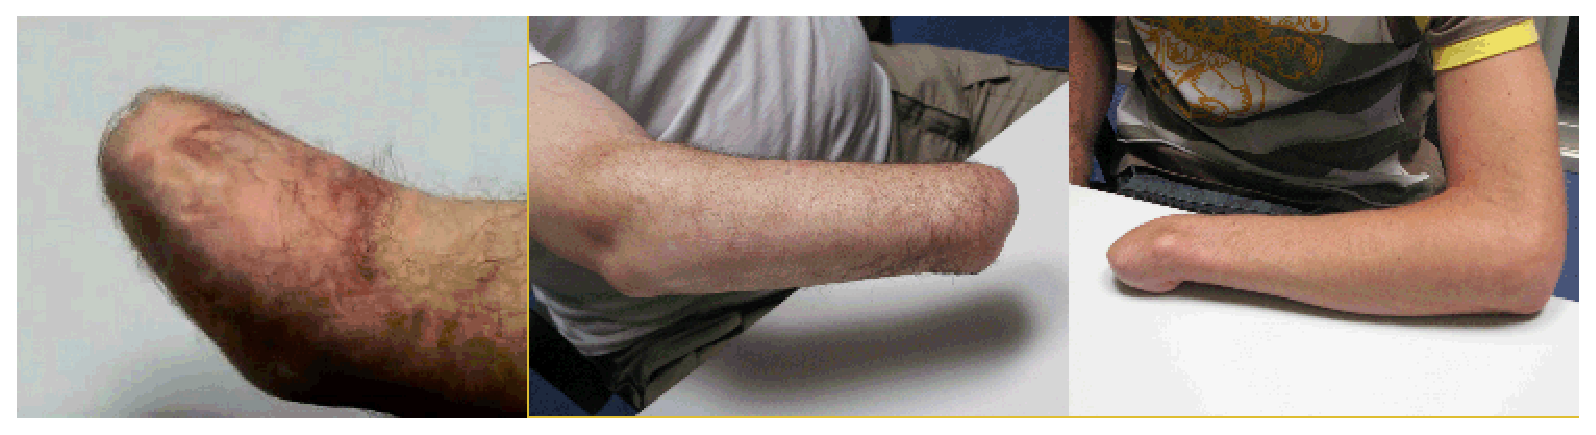
\includegraphics[width=\textwidth]{stumps}
  \caption{the subjects' stumps. Subject $1$ (left) has a trans-radial
    one-third proximal amputation, with a stump about $9$cm long;
    Subject $2$ (center) is trans-radial one-third distal, stump about $20$cm
    long; Subject $3$ (right) is trans-carpal, retaining the full forearm.}
  \label{fig:stumps}
\end{figure}

\begin{figure}
%  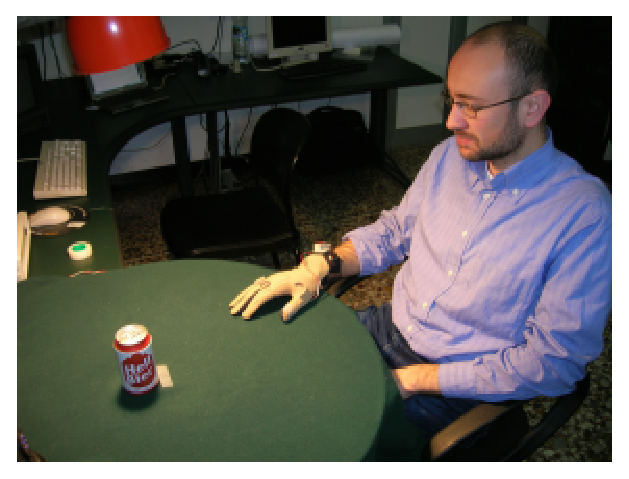
\includegraphics[width=\textwidth]{setup}
  \caption{parts of the experimental setup. (left to right) the FUTEK LMD500
    Hand Gripper; an Otto Bock Myobock EMG electrode; placement of the electrodes
    on a subject's stump, parallel to the forearm axis, equally spaced, held in
    place by an elastic band --- the electrodes' wires are clearly seen.}
  \label{fig:setup}
\end{figure}

\begin{figure}
%  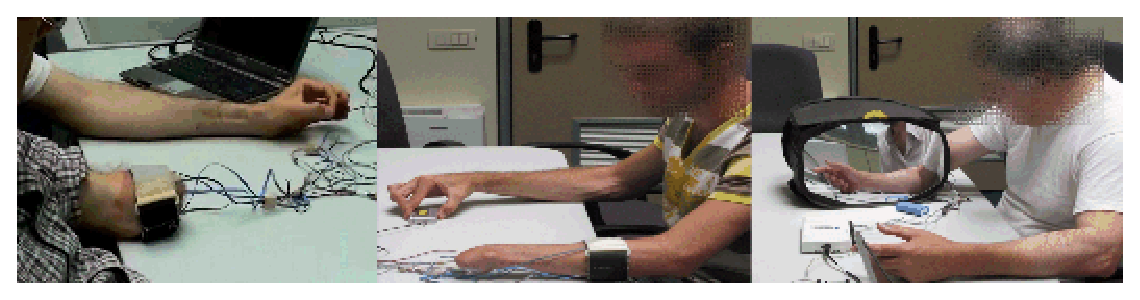
\includegraphics[width=\textwidth]{modalities}
  \caption{the three training modalities. (left to right) Subject $1$
    imitating a pinch grip; Subject $3$ bilaterally performing a pinch
    grip; Subject $2$ assuming the pointing index posture while
    looking in the mirror-box.}
  \label{fig:modalities}
\end{figure}

\begin{figure}
%  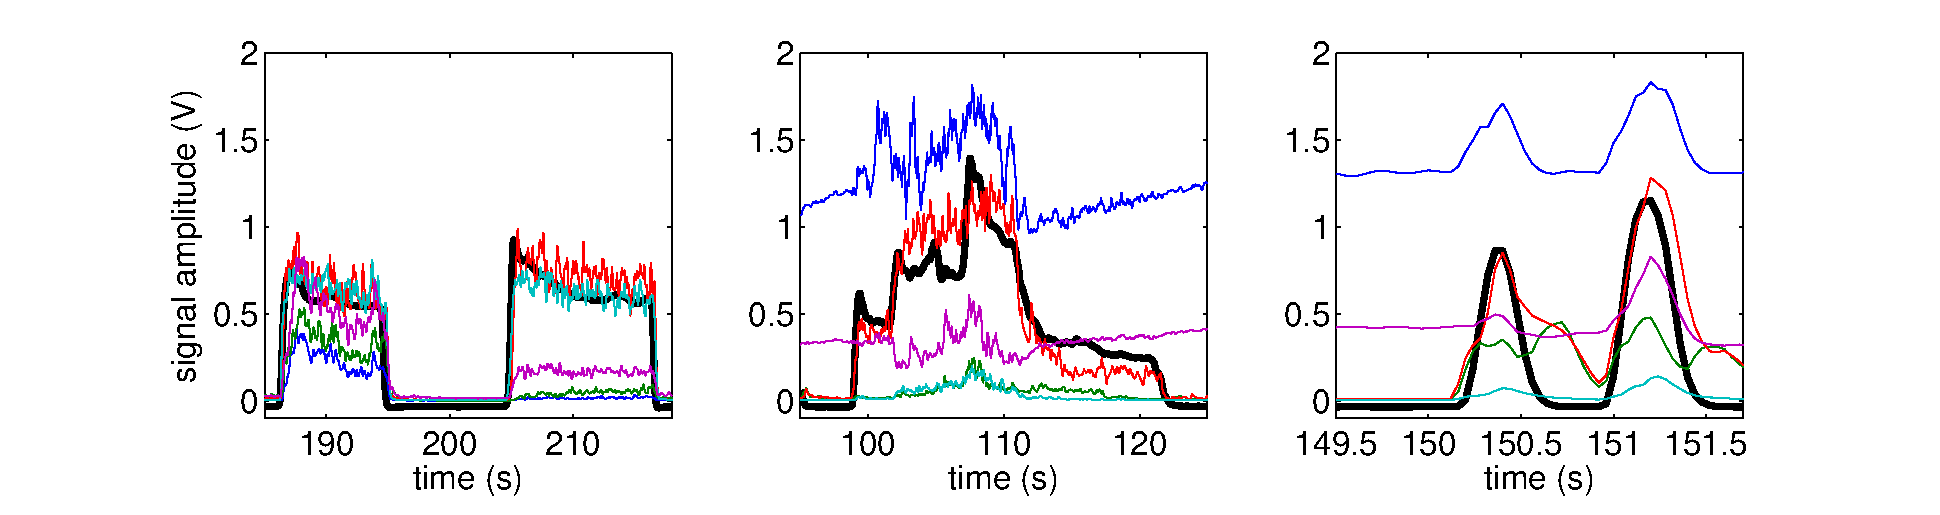
\includegraphics[width=\textwidth]{figExamples}
  \caption{three examples of force (black thick line) and EMG
    signals (coloured thin lines). (left panel) Subject $1$ in the teacher imitation
    modality switches from \po\ to \pw\ at about $200$ seconds of activity --- notice
    the sharp change in relative average magnitude of the EMG signals, before and after
    the switch. (center and right panels) Subject $3$ in the mirror-box modality, slow
    and fast power grasping.}
  \label{fig:examples}
\end{figure}

\begin{figure}
%  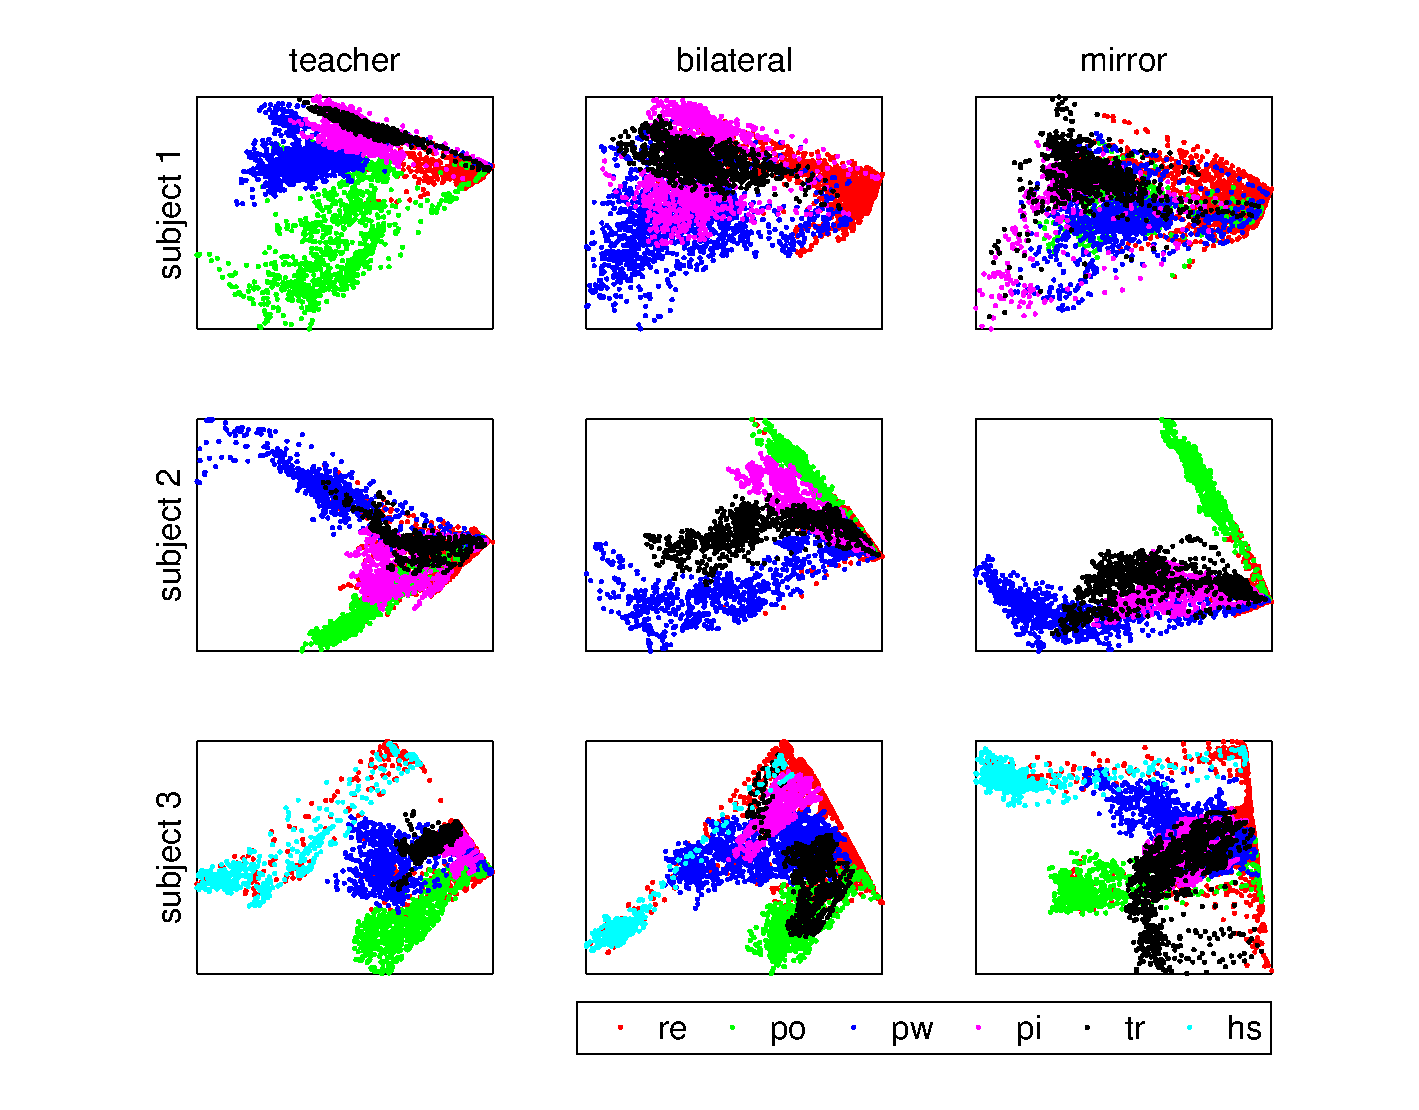
\includegraphics[width=\textwidth]{figPCA}
  \caption{visualisation of the PCA-reduced EMG signals.}
  \label{fig:PCA}
\end{figure}

\begin{figure}
%  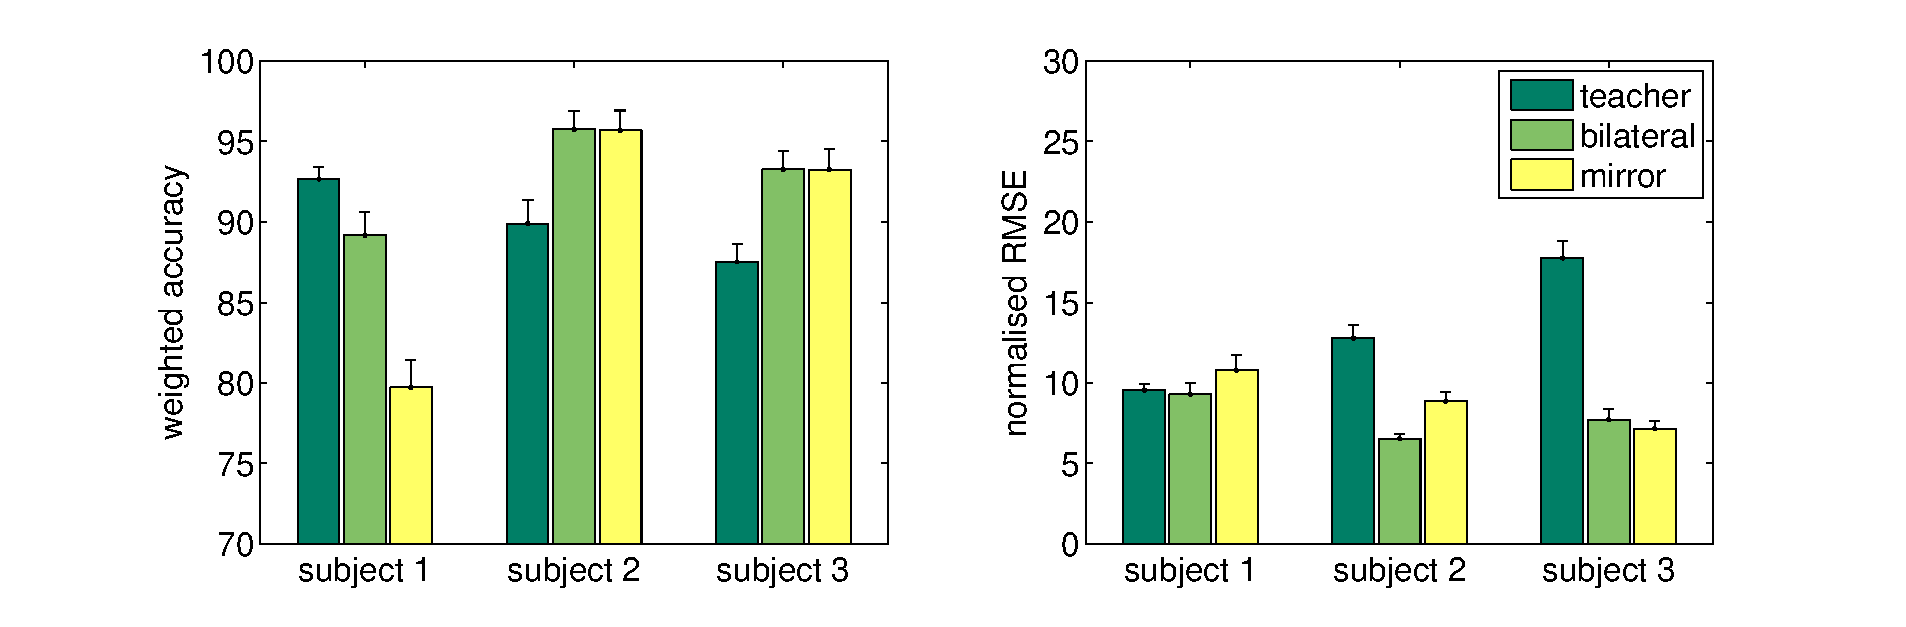
\includegraphics[width=\textwidth]{figPerf}
  \caption{classification (left) and regression (right) performance
    for each subject and modality. Histogram bars are mean values over
    the $10$ splits of the outer cross-validation, error bars denote one
    standard deviation.}
  \label{fig:results}
\end{figure}

\begin{figure}
%  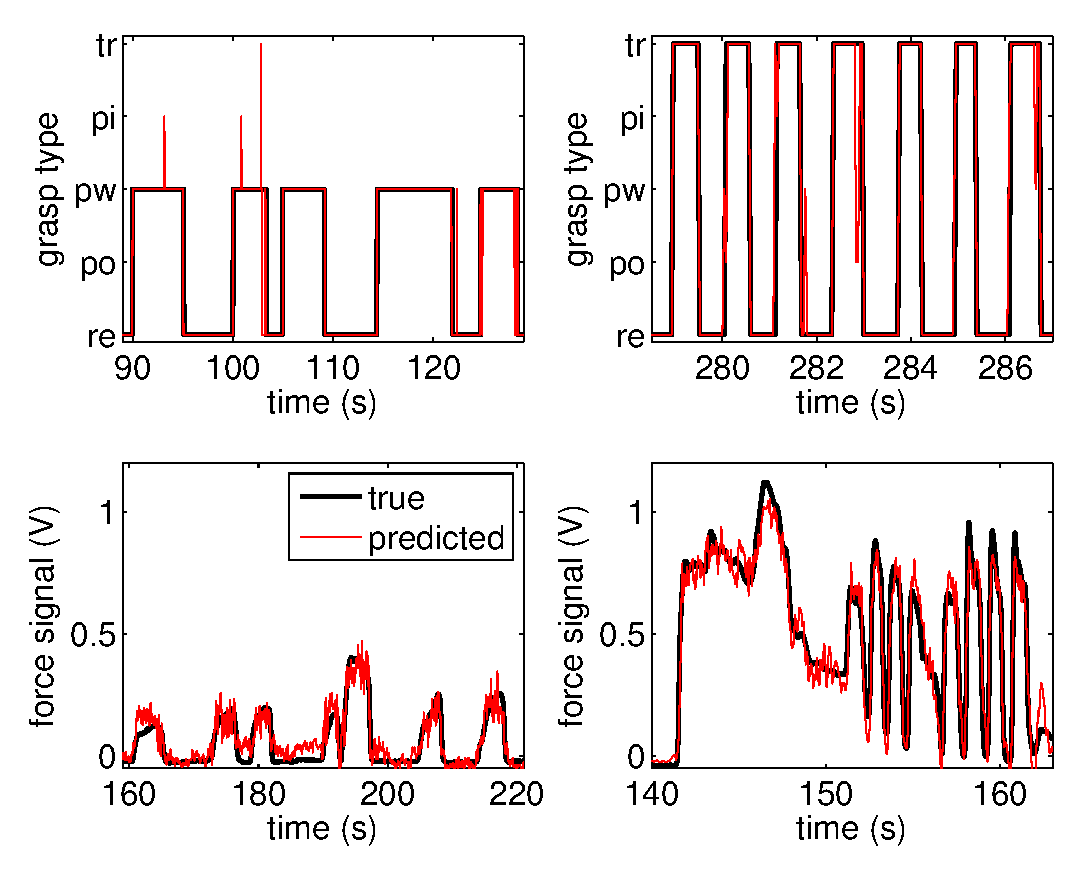
\includegraphics[width=\textwidth]{figGuess}
  \caption{comparing true and predicted targets. (upper row) Classification
    of Subject $2$ in bilateral action (left, weighted accuracy $95.74\% \pm
    1.15\%$) and Subject $1$ in mirror-box (right, $79.72\% \pm 1.70\%$).
    (lower row) Regression of Subjects $2$ (left, normalised RMSE $6.54\% \pm
    0.31\%$) and $3$ (right, $7.70\% \pm 0.65\%$) in bilateral action.}
  \label{fig:guess}
\end{figure}

\begin{figure}
%  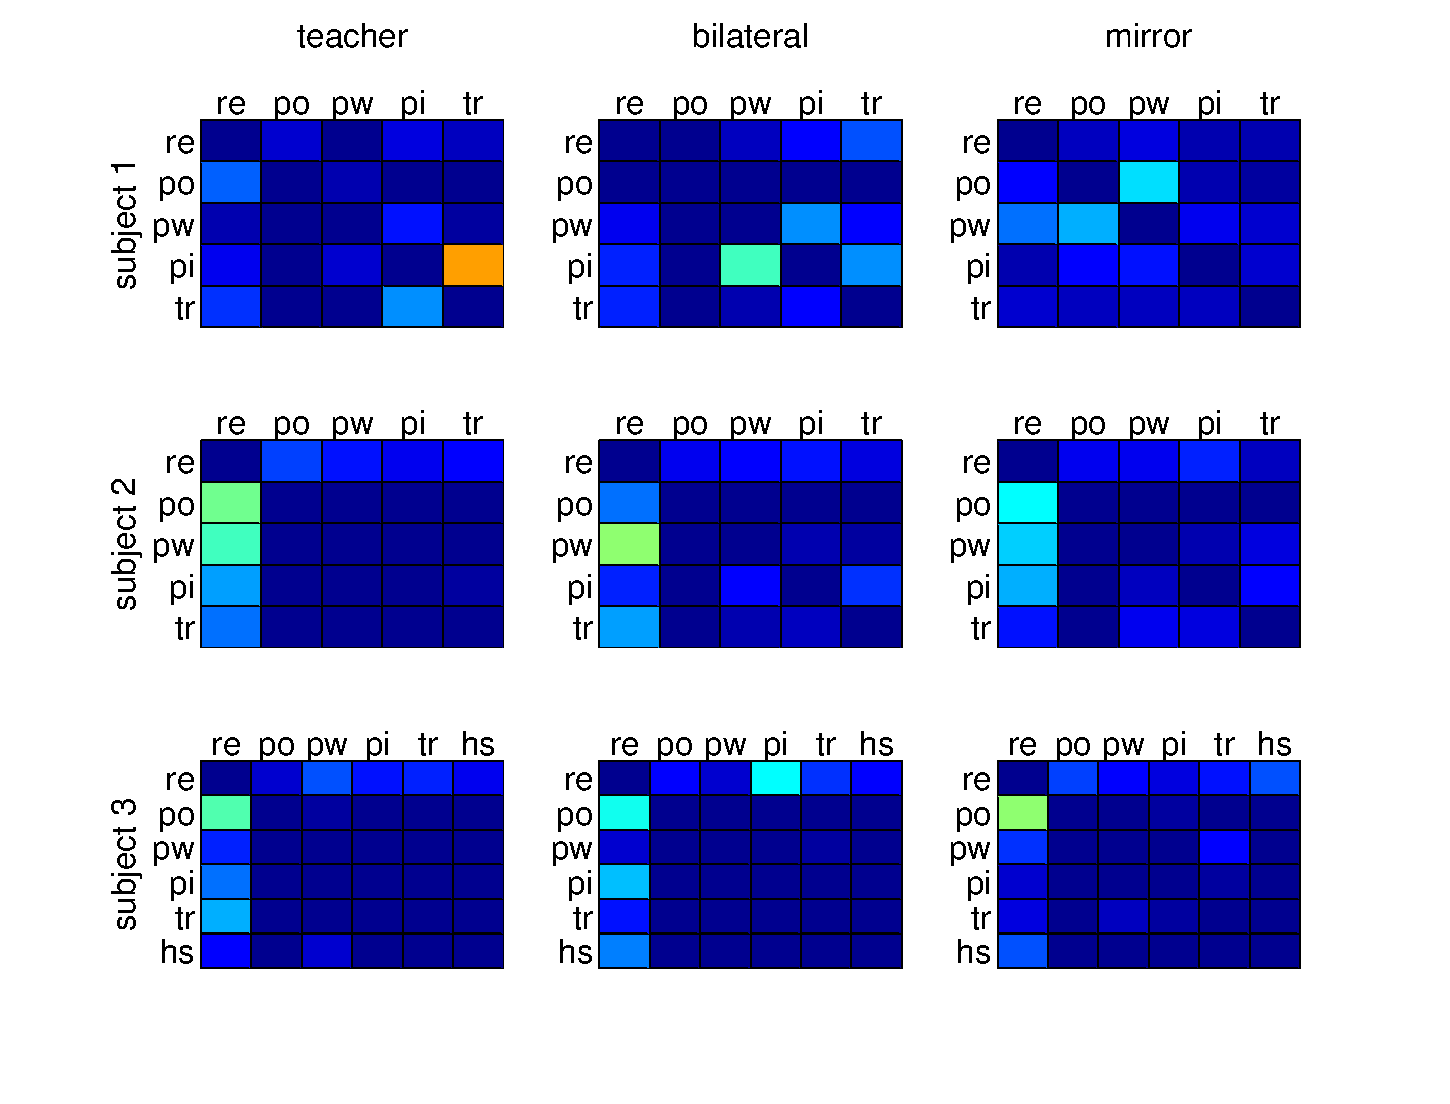
\includegraphics[width=\textwidth]{figConf}
  \caption{confusion matrices for each subject and modality.
    In each matrix $C$, $C_{ij}$ denotes the fraction of labels
    $i$ which have been mistaken for $j$ over the total mistaken
    labels of that particular cycle. The diagonals of the matrices
    are obviously identically zero. Each matrix is the average of
    ten matrices, obtained from each outer cross-validation split.}
  \label{fig:confusion}
\end{figure}

\begin{figure}
%  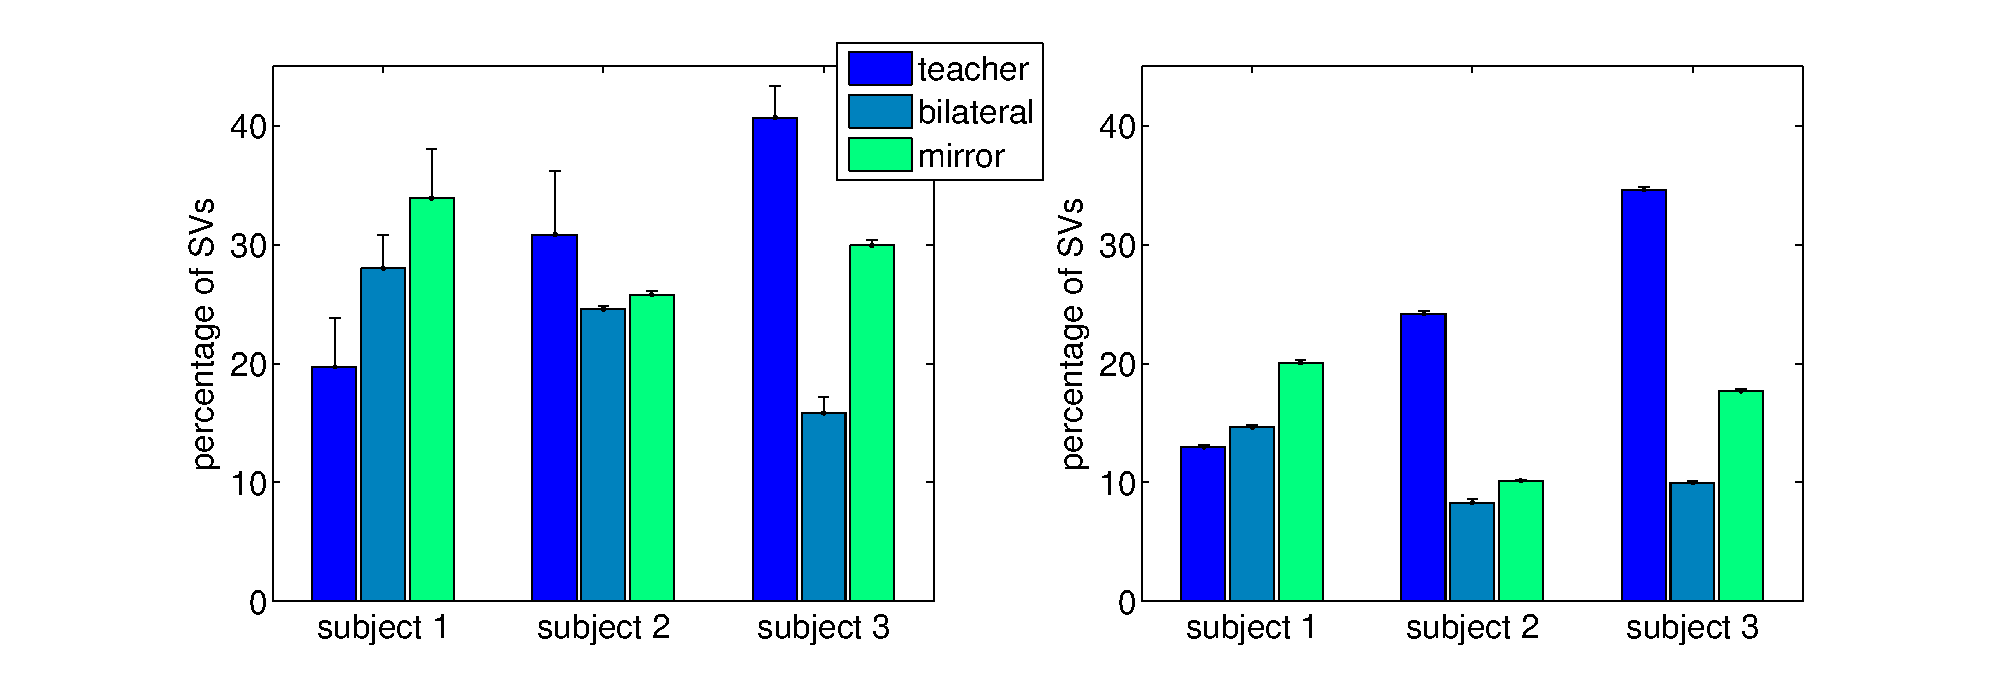
\includegraphics[width=\textwidth]{figSVs}
  \caption{percentages of Support Vectors obtained in the optimal models
  	for classification (left) and regression (right) for each subject and modality.
    Histogram bars are mean values over the $10$ splits of
    the outer cross-validation, error bars denote one standard deviation.}
  \label{fig:SVs}
\end{figure}

%\clearpage
%
%\begin{figure}[htp]
%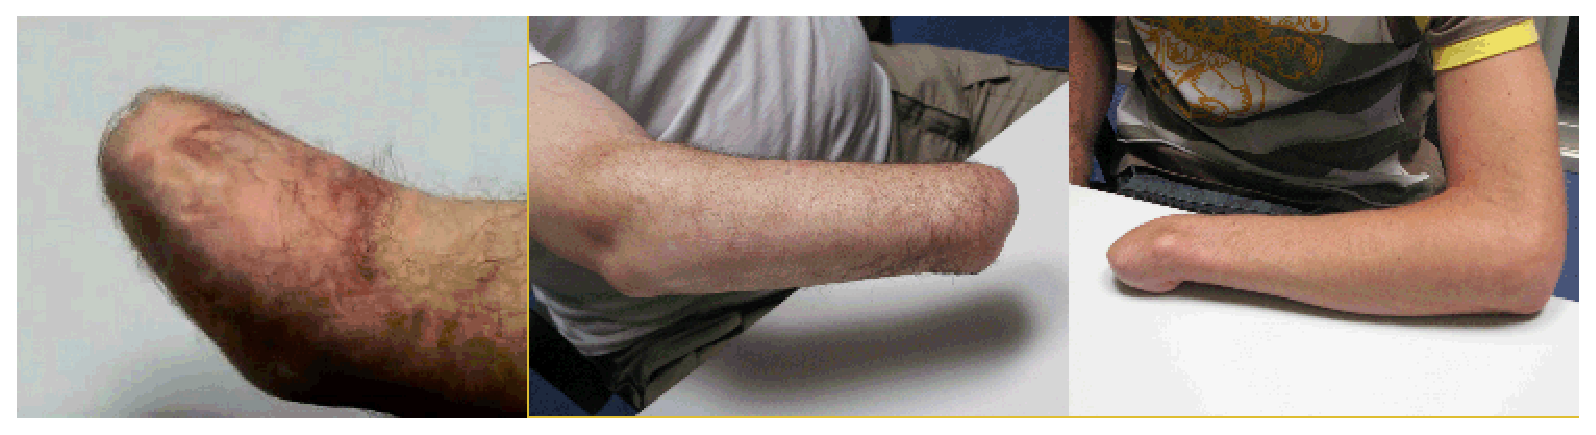
\includegraphics[width=\textwidth]{1-stumps}
%\end{figure}
%
%\clearpage
%
%\begin{figure}[htp]
%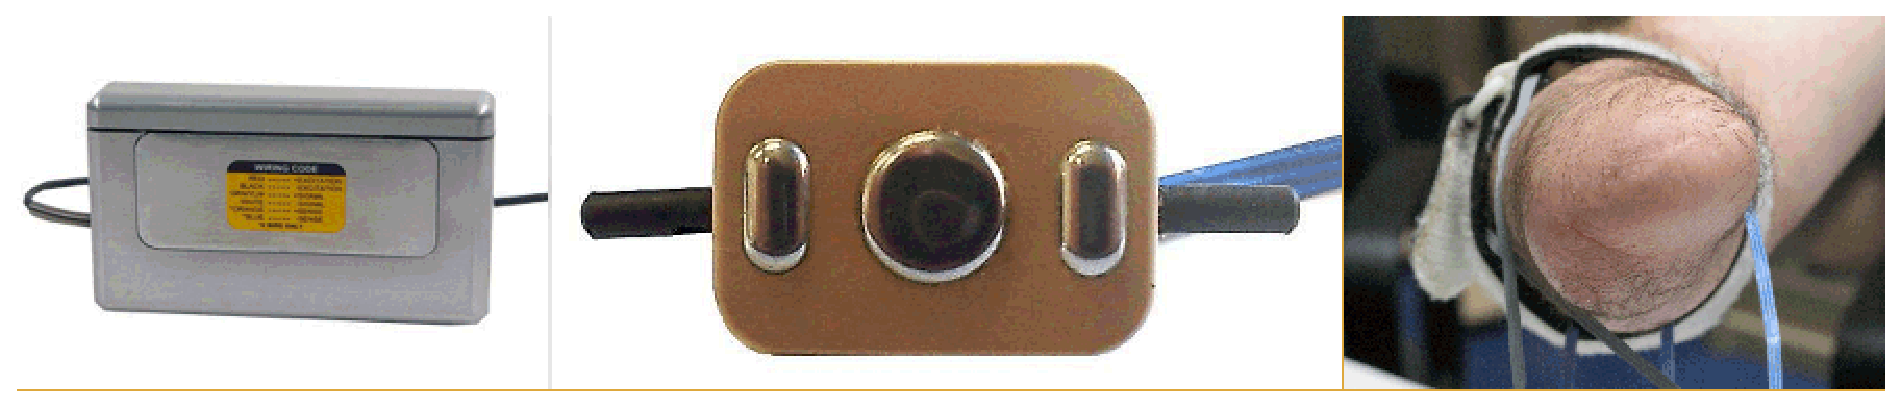
\includegraphics[width=\textwidth]{2-setup}
%\end{figure}
%
%\clearpage
%
%\begin{figure}[htp]
%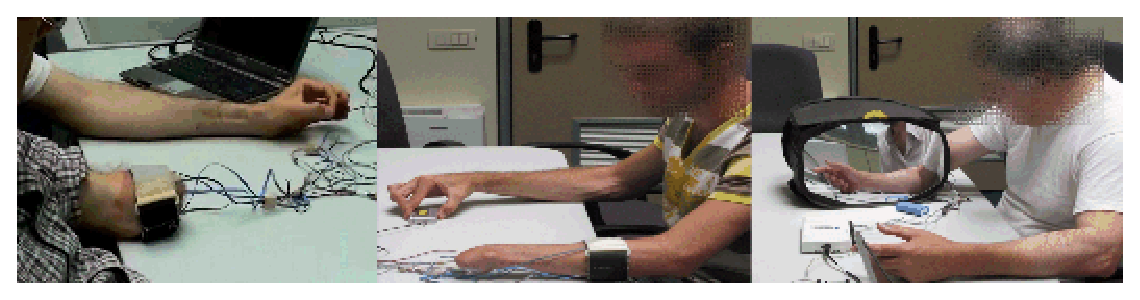
\includegraphics[width=\textwidth]{3-modalities}
%\end{figure}
%
%\clearpage
%
%\begin{figure}[htp]
%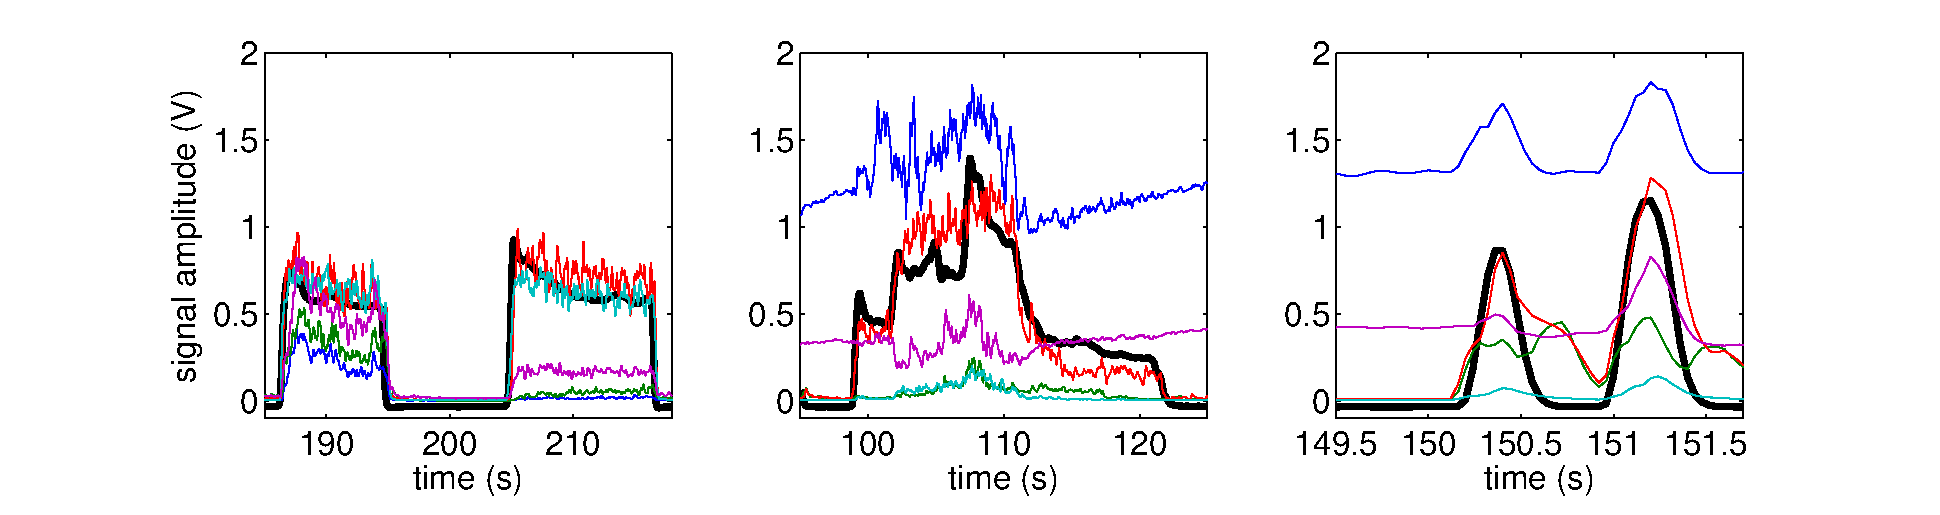
\includegraphics[width=\textwidth]{4-figExamples}
%\end{figure}
%
%\clearpage
%
%\begin{figure}[htp]
%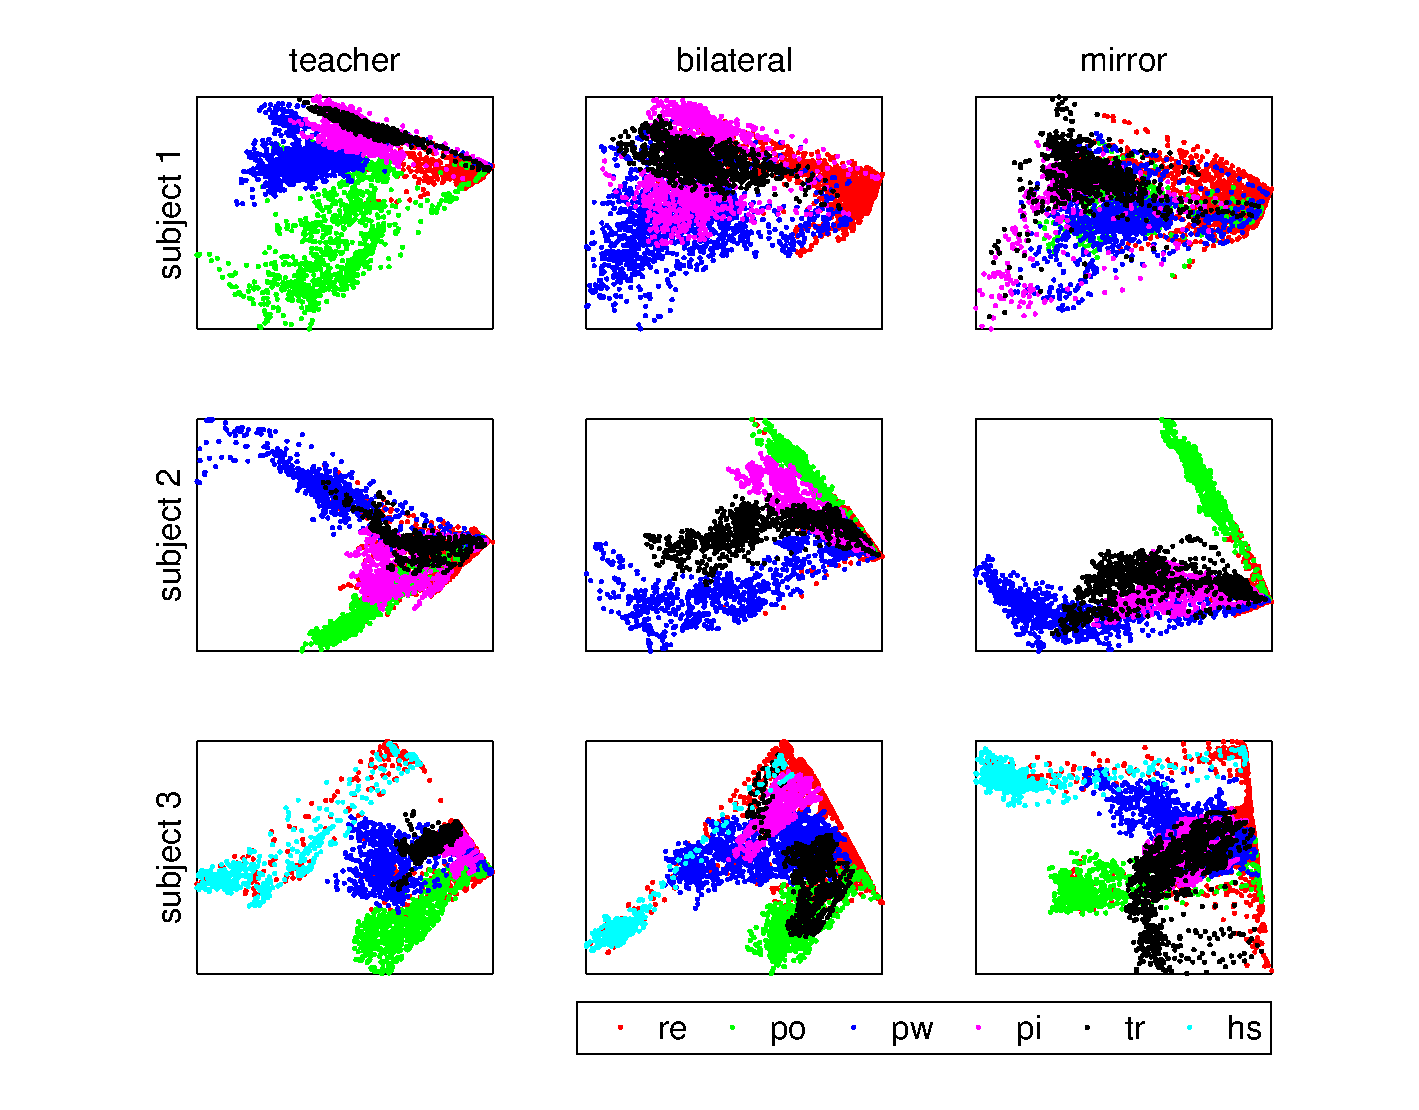
\includegraphics[width=\textwidth]{5-figPCA}
%\end{figure}
%
%\clearpage
%
%\begin{figure}[htp]
%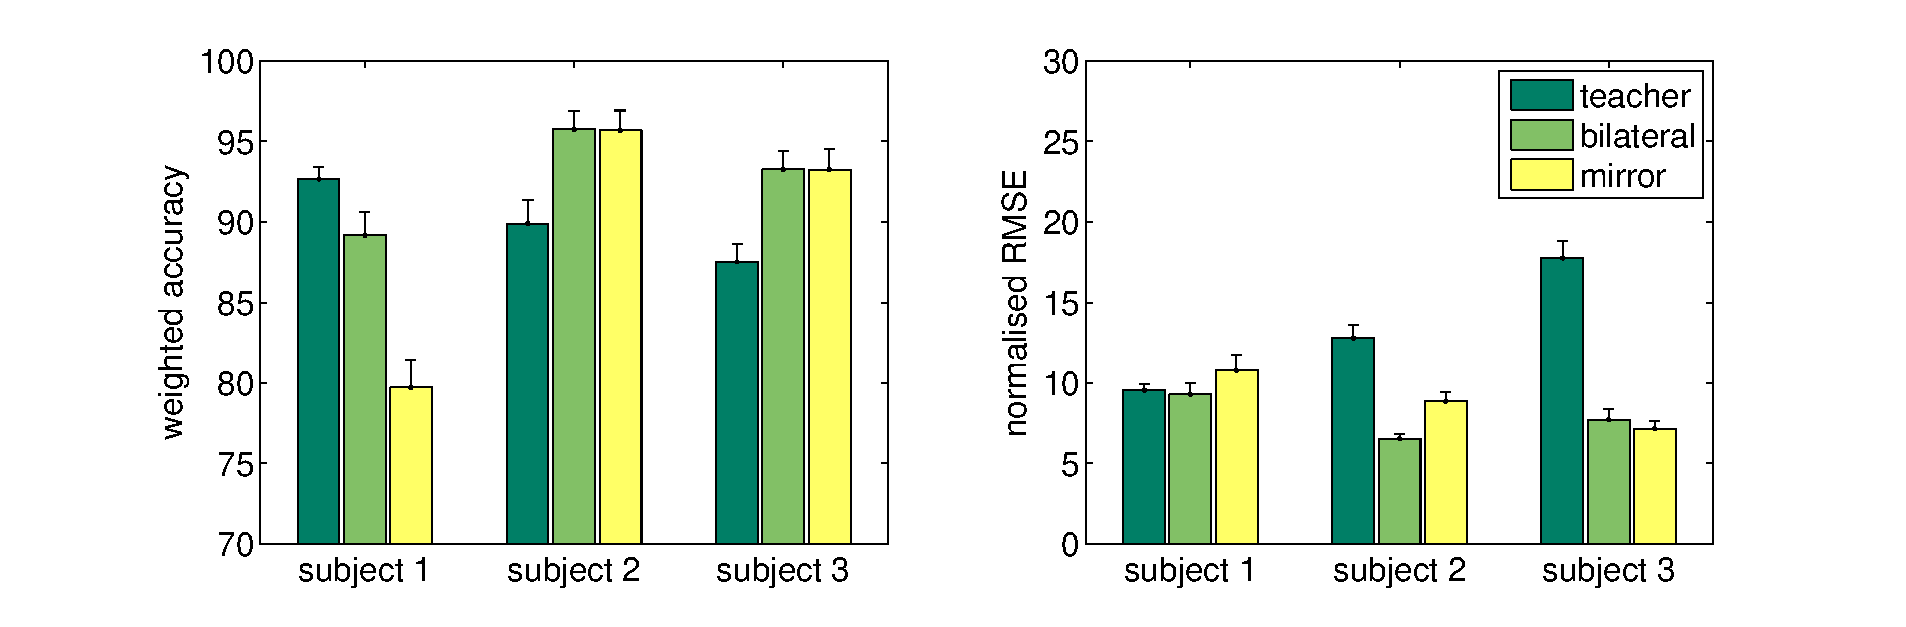
\includegraphics[width=\textwidth]{6-figPerf}
%\end{figure}
%
%\clearpage
%
%\begin{figure}[htp]
%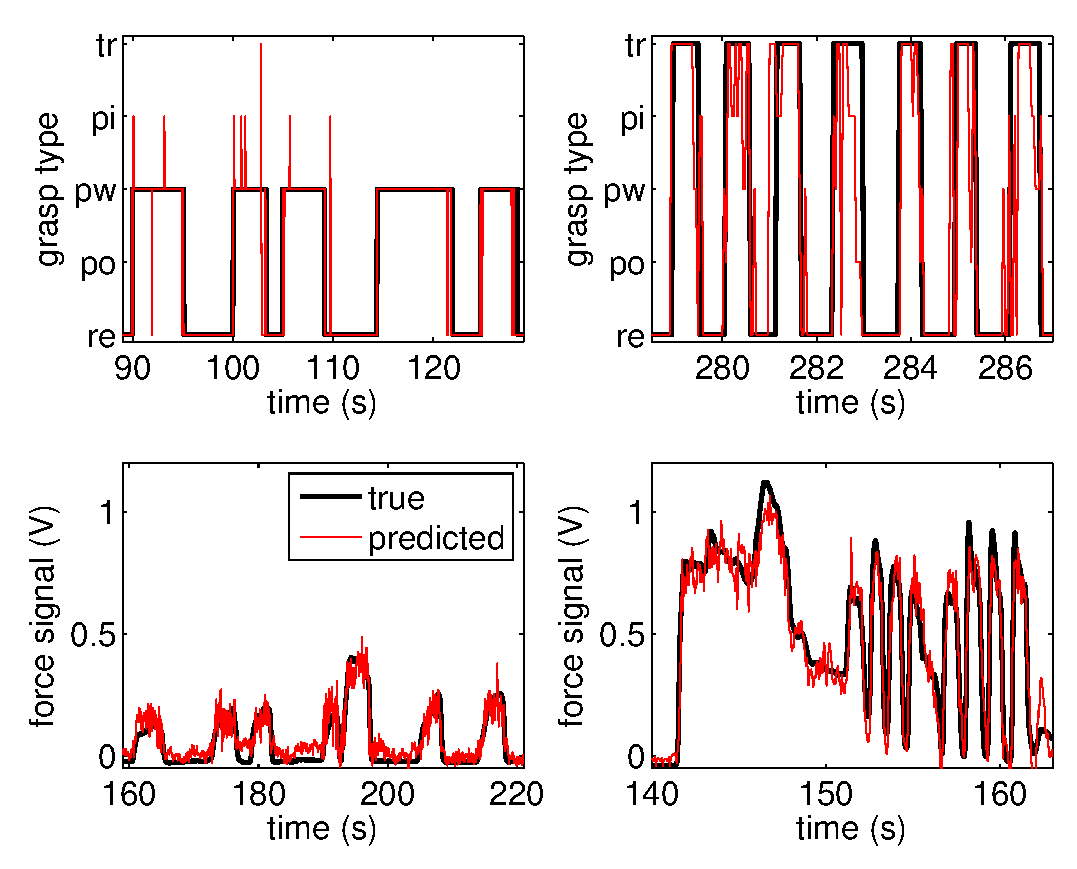
\includegraphics[width=\textwidth]{7-figGuess}
%\end{figure}
%
%\clearpage
%
%\begin{figure}[htp]
%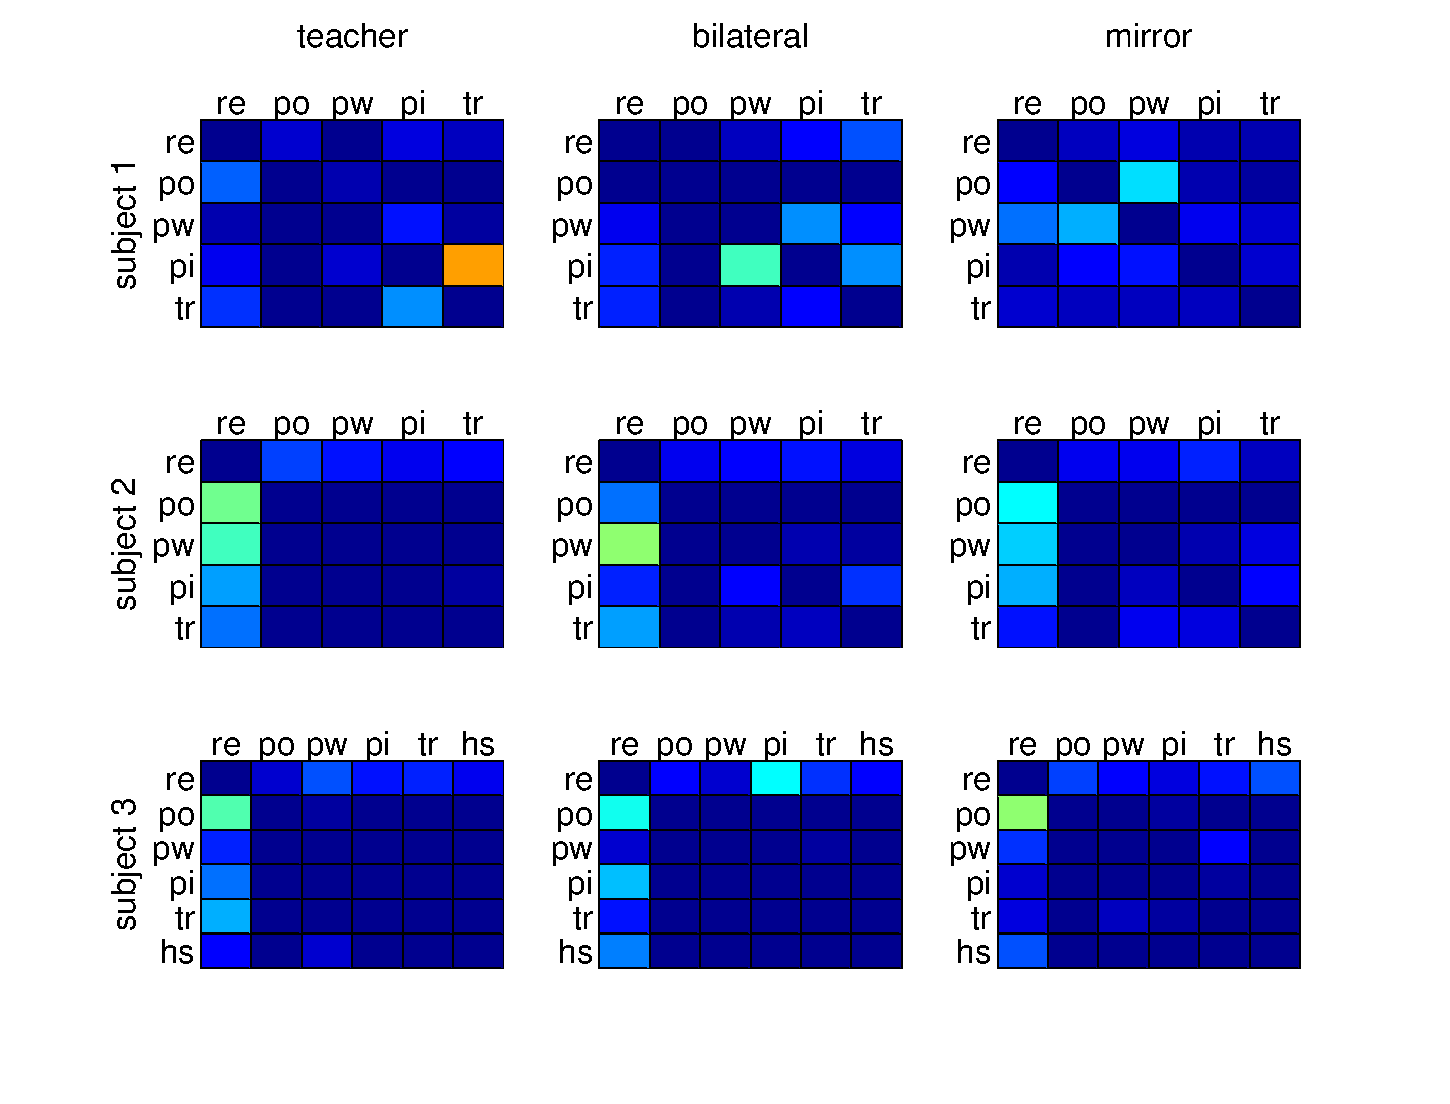
\includegraphics[width=\textwidth]{8-figConf}
%\end{figure}
%
%\clearpage
%
%\begin{figure}[htp]
%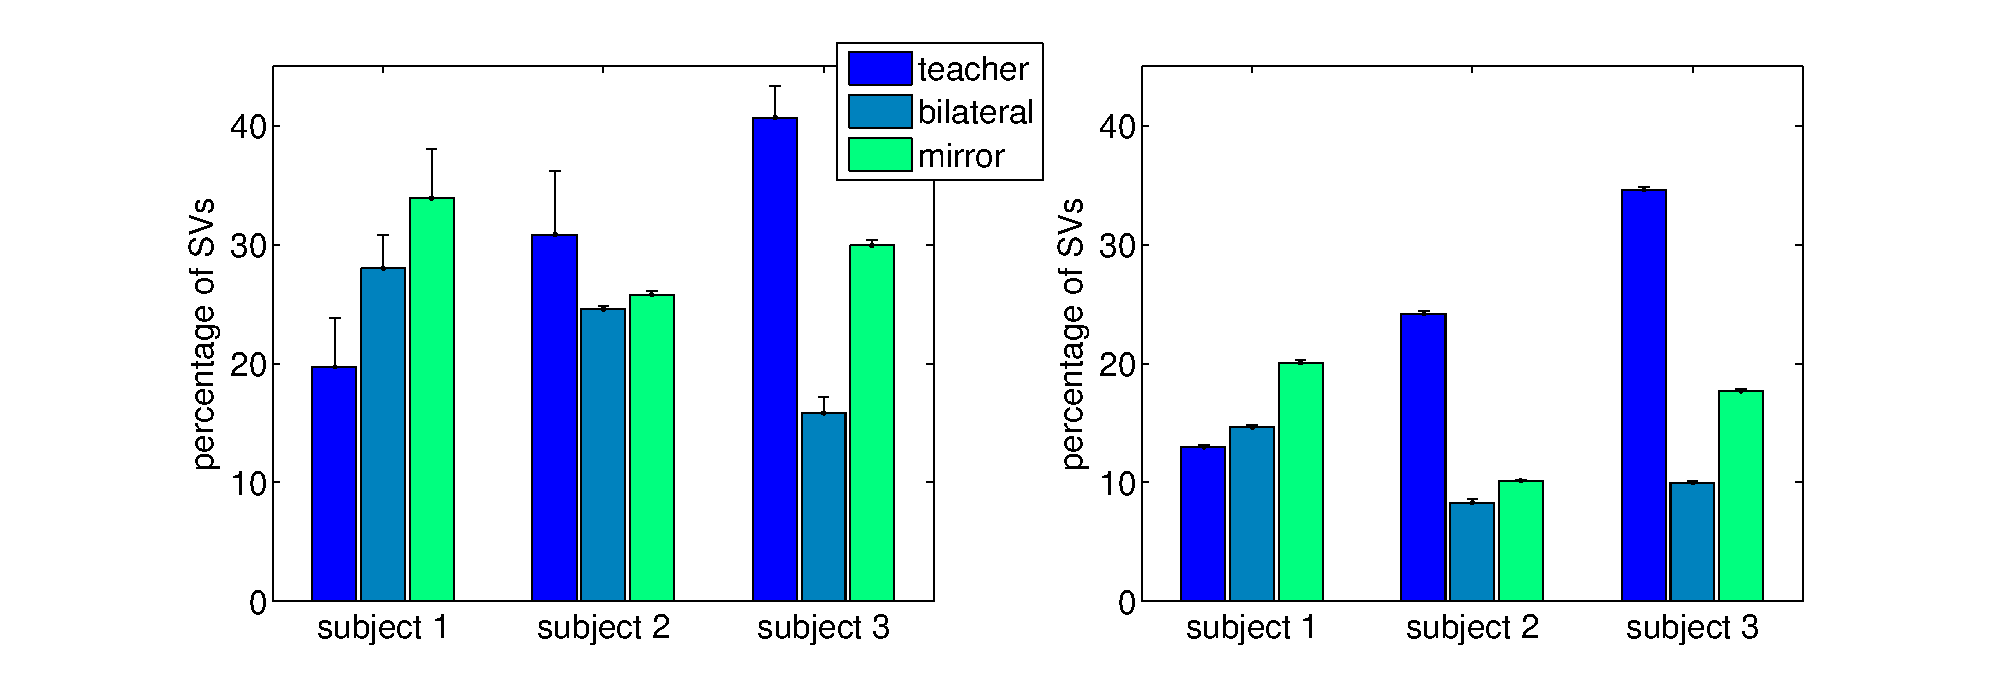
\includegraphics[width=\textwidth]{9-figSVs}
%\end{figure}

\end{document}
